\documentclass[11pt,a4paper]{article}

% === Language and encoding ===
\usepackage[utf8]{inputenc}
% Font encoding: using default OT1 with scalable CM fonts
\usepackage[english]{babel}

% === Mathematics ===
\usepackage{amsmath,amssymb,amsthm}

% === Formatting ===
\usepackage[margin=2.5cm]{geometry}
% microtype omitted for compatibility
\usepackage{booktabs}
\usepackage{float}
\usepackage{graphicx}
\usepackage[dvipsnames]{xcolor}
\usepackage{tikz}
\usetikzlibrary{patterns,arrows.meta,decorations.pathreplacing}
\usepackage[ruled,vlined,linesnumbered]{algorithm2e}
\usepackage{hyperref}
\hypersetup{colorlinks=true,linkcolor=blue!60!black,citecolor=blue!60!black,urlcolor=blue!60!black}

% === Theorems ===
\newtheorem{definition}{Definition}[section]
\newtheorem{proposition}{Proposition}[section]
\newtheorem{theorem}{Theorem}[section]
\newtheorem{corollary}{Corollary}[section]
\newtheorem{lemma}{Lemma}[section]
\theoremstyle{remark}
\newtheorem{remark}{Remark}[section]
\newtheorem{hypothesis}{Hypothesis}[section]
\newtheorem{principle}{Design Principle}[section]

% === Custom commands ===
\newcommand{\R}{\mathbb{R}}
\newcommand{\E}{\mathbb{E}}
\newcommand{\Syn}{\mathrm{Syn}}
\newcommand{\Red}{\mathrm{Red}}
\newcommand{\Unq}{\mathrm{Unq}}
\newcommand{\MI}{\mathrm{I}}
\newcommand{\KL}{\mathrm{D_{KL}}}

\title{%
  \textbf{CasIA: Breaking the Self-Validation Ceiling} \\[0.5em]
  \large A Structural Solution to Monolithic LLM Blind Spots \\
  using Partial Information Decomposition
}

\author{
  C\'esar Lacruz \\
  \texttt{Project Director} \\[0.3em]
  \small Working Paper --- March 2026 (v12 -- preprint)
}

\date{}

\begin{document}
\maketitle

% ============================================================
% ABSTRACT
% ============================================================
\begin{abstract}
Current LLMs face a fundamental information-theoretic limit: any self-validation mechanism operating within the same representational space cannot reliably detect its own systematic errors (Proposition \ref{prop:bound}). This ceiling persists under stochastic sampling and extends to \emph{all} self-interactive protocols, including self-consistency and multi-agent debate within a single model (Theorem \ref{thm:transcript}). Even if iterative test-time computation expands the effective representational space beyond single-pass encoding, the ceiling remains a function of the model's parameters alone (Appendix \ref{sec:dynamic}).

We introduce \textbf{CasIA}, a principled architecture that structurally separates generation, metacognitive validation, and normative regulation into independent parameter spaces---applying privilege separation to AI safety. Success is measured by \emph{synergy} via Partial Information Decomposition (PID): information about correctness that exists only in the combination of components, never in any one alone. We prove that systematic errors invisible to self-validation become detectable under cross-model validation when representations are complementary (Proposition \ref{prop:error_detect}), and derive a Bayes error floor showing that no classifier built on a model's own outputs can overcome this limit in its blind spots (Lemma \ref{lem:fano}). CasIA raises the ceiling by combining independently expanded representational spaces---benefiting from dynamic expansion within each component while adding structural separation across them. We provide a complete experimental protocol---with matched-compute baselines, poisoned-context stress tests, and pre-registered PID robustness criteria---to quantify the ``complementarity gap'' of today's frontier models. CasIA requires no new theoretical breakthroughs and can be instantiated today with off-the-shelf models.
\end{abstract}

\vspace{0.5em}
\noindent\textbf{Keywords:} Multi-model architecture, Partial Information Decomposition, synergy, AI safety, privilege separation, structural metacognition, multi-agent systems.

\begin{figure}[ht]
\centering
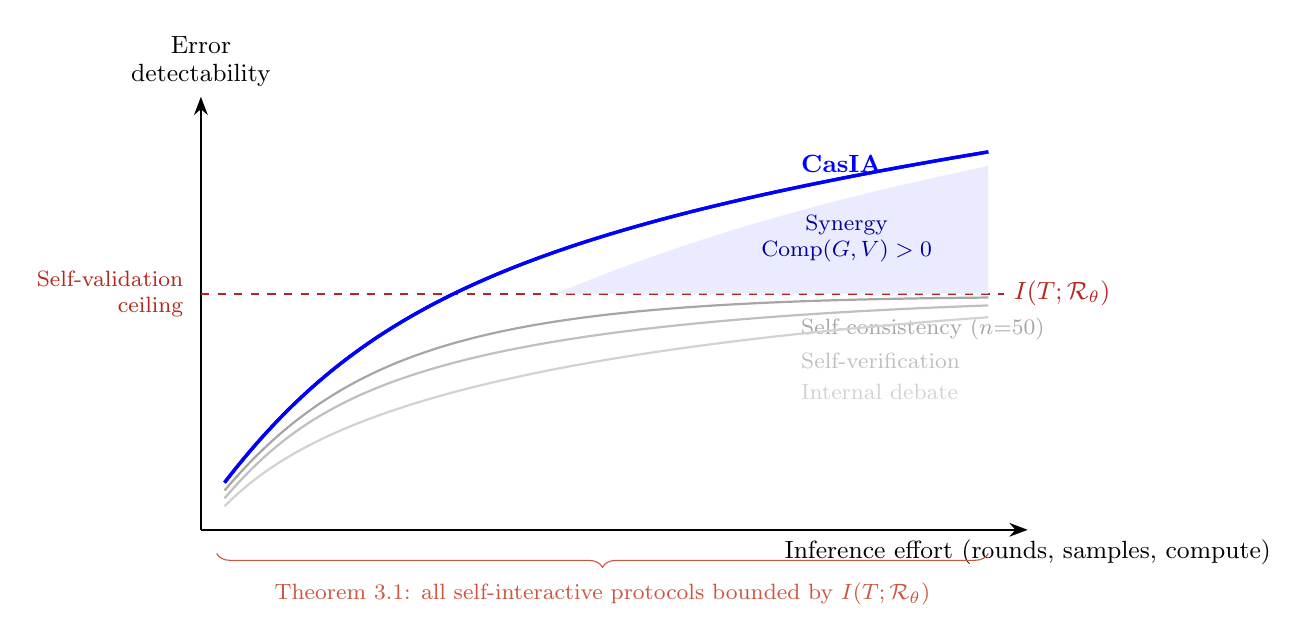
\begin{tikzpicture}[>=Stealth, scale=1.0]
  % Axes
  \draw[->, thick] (0,0) -- (10.5,0) node[below] {\small Inference effort (rounds, samples, compute)};
  \draw[->, thick] (0,0) -- (0,5.5) node[above, align=center] {\small Error\\[-2pt]\small detectability};
  
  % Ceiling line
  \draw[dashed, BrickRed, thick] (0,3.0) -- (10.2,3.0);
  \node[right, BrickRed, font=\small\bfseries] at (10.2,3.0) {$I(T; \mathcal{R}_\theta)$};
  \node[left, BrickRed, font=\footnotesize, align=right] at (-0.1,3.0) {Self-validation\\ceiling};
  
  % Monolithic curves (all hit ceiling)
  \draw[gray!70, thick] (0.3,0.5) .. controls (2,2.5) and (4,2.9) .. (10,2.95);
  \node[gray!70, font=\footnotesize, right] at (7.5,2.55) {Self-consistency ($n{=}50$)};
  
  \draw[gray!50, thick] (0.3,0.4) .. controls (1.5,1.8) and (3,2.6) .. (10,2.85);
  \node[gray!50, font=\footnotesize, right] at (7.5,2.15) {Self-verification};
  
  \draw[gray!35, thick] (0.3,0.3) .. controls (1.2,1.2) and (3,2.2) .. (10,2.7);
  \node[gray!35, font=\footnotesize, right] at (7.5,1.75) {Internal debate};
  
  % CasIA curve (breaks ceiling)
  \draw[Blue, very thick] (0.3,0.6) .. controls (2,2.8) and (4,3.8) .. (10,4.8);
  \node[Blue, font=\small\bfseries, right] at (7.5,4.65) {CasIA};
  
  % Annotation: synergy region
  \fill[Blue!8] (4.5,3.0) -- (10,3.0) -- (10,4.62) .. controls (7,4.0) and (5.5,3.4) .. (4.5,3.0);
  \draw[Blue, very thick] (0.3,0.6) .. controls (2,2.8) and (4,3.8) .. (10,4.8);
  \node[Blue!60!black, font=\footnotesize, align=center] at (8.2,3.7) {Synergy\\$\mathrm{Comp}(G,V) > 0$};
  
  % Bracket for monolithic region
  \draw[decorate, decoration={brace, amplitude=5pt, mirror}, BrickRed!70] (0.2,-0.3) -- (10,-0.3);
  \node[BrickRed!70, font=\footnotesize, below] at (5.1,-0.55) {Theorem 3.1: all self-interactive protocols bounded by $I(T; \mathcal{R}_\theta)$};
\end{tikzpicture}
\caption{The self-validation ceiling. Monolithic methods (gray curves) asymptotically approach the information-theoretic bound $I(T; \mathcal{R}_\theta)$ regardless of the number of rounds, samples, or sophistication of the protocol (Theorem \ref{thm:transcript}). CasIA (blue) breaks the ceiling by introducing a complementary representation space $\mathcal{R}_{\theta_V}$ with $\mathrm{Comp}(G, V) > 0$. The shaded region represents synergistic information---detectable only through structural separation.}
\label{fig:ceiling}
\end{figure}

\vspace{0.5em}

% ============================================================
% 1. INTRODUCTION
% ============================================================
\section{Introduction}
\label{sec:intro}

No intelligent biological system relies on a single neural circuit to both generate a response \emph{and} validate it. Evolution discovered this millions of years ago: the prefrontal cortex does not evaluate its own decisions---the amygdala, the cerebellum, the basal ganglia intervene, each with distinct connectivity, learning history, and neurochemical substrate. The robustness of the brain stems not from the power of any single structure, but from the \emph{productive tension} between independent structures that process the same information in complementary ways.

The AI industry has spent the last decade pretending this doesn't matter. This paper proves it does---and shows how to fix it.

The problem is structural, not quantitative. If the generation process $G$ and the validation process $V$ share parameters $\theta$, then $V$ is subject to the same representational limitations as $G$. A model that ``does not know what it does not know'' cannot discover it by interrogating itself with the same tools that produced the ignorance. Adding more parameters to the same latent space does not solve this problem---it deepens it, because it expands the capacity to generate sophisticated errors without expanding the capacity to detect them from outside that space.

The question motivating this work is not \emph{how to make models larger}, but \emph{how to make existing models compensate each other in ways that none could achieve alone}. And, crucially, how to \emph{measure} whether they are succeeding. Our approach applies a well-established principle from distributed systems security---\emph{privilege separation}---to AI architecture: the safety of an intelligent system should be a structural property, not merely a training outcome. A compromised process cannot escalate privileges when the authentication system resides in independent memory space. CasIA applies this logic to generation and validation: a manipulated generator cannot corrupt a validator that shares no representational space with it.

Our goal is not to propose yet another prompting heuristic, but to provide a testable architectural principle: when does combining existing models yield strictly new information about task correctness, and under what stability conditions?

\subsection{Contributions}

This work makes seven contributions:

\begin{enumerate}
  \item \textbf{Formalization of the monolithic self-validation problem} (Section \ref{sec:problem}): we show that the mutual information between a model's generation and self-validation is upper-bounded by a function of the internal representational diversity, and that this bound holds under stochastic sampling.
  
  \item \textbf{Generalization to self-interactive protocols} (Section \ref{sec:problem}): we prove that the self-validation ceiling extends to arbitrary multi-round self-interactive protocols, including self-consistency, multi-turn self-verification, and internal debate (Theorem \ref{thm:transcript}).
  
  \item \textbf{Detectability bound} (Section \ref{sec:problem}): via Fano's inequality, we derive a lower bound on the error rate of any classifier built on a model's own outputs in its systematic error region, connecting the information-theoretic ceiling to a measurable operational limit (Lemma \ref{lem:fano}).
  
  \item \textbf{Error detectability under cross-validation} (Section \ref{sec:problem}): we prove that systematic errors undetectable by self-validation become diagnosable when a validator with complementary representation space is introduced.
  
  \item \textbf{CasIA architecture} (Section \ref{sec:architecture}): we propose a three-component system with structural separation of generation, metacognitive validation, and normative regulation---the minimum configuration that separates all three concerns without collapsing functions.
  
  \item \textbf{PID synergy criterion} (Section \ref{sec:formal}): we formally define when a multi-model system exhibits measurable synergistic coordination, using Partial Information Decomposition.
  
  \item \textbf{Stability analysis and experimental protocol} (Sections \ref{sec:stability}--\ref{sec:experiments}): we derive sufficient conditions for feedback loop convergence (including a formal contraction result under linear feedback, Proposition \ref{prop:linear_contraction}) and propose reproducible experiments with matched-compute monolithic baselines and poisoned-context stress tests.
\end{enumerate}

% ============================================================
% 2. RELATED WORK
% ============================================================
\section{Related Work}
\label{sec:related}

The intuition that a single model is not enough is not new. What has been missing is a formal framework that defines \emph{when} the combination of models produces something genuinely distinct from the sum of its parts, and \emph{how to measure it}. We review existing approaches and their relationship to CasIA.

\paragraph{Self-validation in LLMs.}
Self-consistency \cite{wang2023selfconsistency} and chain-of-thought verification \cite{weng2023verification} approaches attempt to improve reliability by sampling multiple reasoning chains and selecting by majority. However, the sampling distribution remains conditioned on the same model, which limits the real diversity of verifications.

\paragraph{Constitutional AI.}
Bai et al. \cite{bai2022constitutional} propose that a model revise its own outputs according to a set of constitutional principles. CasIA extends this idea by assigning normative regulation to a component with independent parameters, eliminating the dependence on self-modification.

\paragraph{Mixture of Experts (MoE).}
Mixture-of-Experts architectures \cite{shazeer2017moe,fedus2022switch} distribute computation among specialized sub-networks, but all experts share the same embedding space and routing layer. From the perspective of Proposition \ref{prop:bound}, MoE remains a single system: the router conditions all expert activations on a shared representation $\mathcal{R}_\theta$, and therefore the self-validation bound applies to the ensemble as a whole. CasIA differs fundamentally: the components share neither parameters, embedding space, nor routing mechanism.

\paragraph{Ensemble Methods.}
Classical ensemble approaches---bagging, boosting, stacking---combine model outputs through static aggregation (e.g., majority voting) or sequential correction. These methods improve accuracy through \emph{diversity of predictions}, but do not incorporate a dynamic feedback loop between components. CasIA can be understood as a recursive, dynamically orchestrated ensemble where the interaction protocol (Algorithm \ref{alg:protocol}) allows components to refine their contributions based on diagnostic signals from other components. The key distinction is that CasIA's synergy criterion (Definition \ref{def:agency}) provides a formal measure of when the ensemble produces genuinely new information, not merely averaged predictions.

\paragraph{Multi-Agent Systems.}
Debate frameworks between models \cite{irving2018debate,du2023multiagent} and cross-verification \cite{cohen2023lmvsverifier} demonstrate empirical improvements when using multiple models. CasIA contributes a formal success criterion (PID synergy) and a stability analysis for the interaction loop.

\paragraph{Partial Information Decomposition.}
Williams and Beer \cite{williams2010pid} introduced PID as a framework for decomposing mutual information into components of redundancy, unique information, and synergy. Subsequent applications in neuroscience \cite{timme2018pid_neuro} have demonstrated its utility for quantifying distributed computation in biological systems. This work, to the best of our knowledge, is the first to propose PID as a success criterion for multi-model AI architectures.

\paragraph{Global Workspace Theory.}
The cognitive architecture of Baars \cite{baars1988cognitive} posits a shared workspace where specialized modules compete and cooperate to produce coherent behavior. CasIA implements a computational version of this idea with formally independent modules.

% ============================================================
% 3. PROBLEM FORMULATION
% ============================================================
\section{The Monolithic Self-Validation Problem}
\label{sec:problem}

Before proposing a solution, it is necessary to demonstrate that the problem exists rigorously, not merely anecdotally. This section formalizes an intuition that many engineers share but that is rarely expressed in verifiable terms: why does a model that ``reviews itself'' have a reliability ceiling it cannot surpass?

\subsection{Preliminary Definitions}

\begin{definition}[Generative Model]
\label{def:model}
Let $\mathcal{M}_\theta$ be an autoregressive model with parameters $\theta \in \Theta$. Given an input context $x \in \mathcal{X}$, $\mathcal{M}_\theta$ defines a conditional distribution $p_\theta(y \mid x)$ over the output space $\mathcal{Y}$.
\end{definition}

\begin{definition}[Self-Validation]
\label{def:selfvalidation}
The self-validation of $\mathcal{M}_\theta$ is the process by which the same model evaluates its own output:
\begin{equation}
  v = \mathcal{M}_\theta(x, y; \pi_v)
\end{equation}
where $\pi_v$ is a validation prompt or instruction, and $y$ is the output previously generated by $\mathcal{M}_\theta(x; \pi_g)$ with generation prompt $\pi_g$. Note that both processes use the same parameters $\theta$.
\end{definition}

\begin{definition}[Accessible Representation Space]
\label{def:rep_space}
For a model $\mathcal{M}_\theta$, we define the \emph{accessible representation space} $\mathcal{R}_\theta \subseteq \R^d$ as the set of activation vectors at the intermediate representation layer that the model can produce for some input in the domain:
\begin{equation}
  \mathcal{R}_\theta = \left\{ h \in \R^d \;\middle|\; \exists\, x \in \mathcal{X} : h = f_\theta(x) \right\}
\end{equation}
where $f_\theta$ denotes the model's intermediate representation function.
\end{definition}

\subsection{Self-Validation Bound}

\begin{proposition}[Self-Validation Upper Bound]
\label{prop:bound}
Let $T$ be a random variable representing response correctness (with $T = 1$ if the response is correct, $T = 0$ otherwise). Let $Y = \mathcal{M}_\theta(X; \pi_g)$ be the generated output and $V = \mathcal{M}_\theta(X, Y; \pi_v)$ the self-validation. Then:
\begin{equation}
  \MI(T; V \mid Y) \leq \MI(T; \mathcal{R}_\theta) - \MI(T; Y)
\end{equation}
That is, the additional information that self-validation can provide about correctness is bounded by the information that the representation space contains about $T$ minus the information already captured in the output.
\end{proposition}

\begin{proof}
By the mutual information chain rule:
\begin{equation}
  \MI(T; Y, V) = \MI(T; Y) + \MI(T; V \mid Y)
\end{equation}

Since both $Y$ and $V$ are deterministic functions of $\mathcal{R}_\theta$ (for a fixed input), by the data processing inequality:
\begin{equation}
  \MI(T; Y, V) \leq \MI(T; \mathcal{R}_\theta)
\end{equation}

Combining both expressions:
\begin{equation}
  \MI(T; V \mid Y) \leq \MI(T; \mathcal{R}_\theta) - \MI(T; Y)
\end{equation}
\end{proof}

\paragraph{Stochasticity and the self-validation bound.} Autoregressive models introduce stochasticity through sampling, but this randomness does not constitute an additional information source about the target variable $T$. Let $Y = f(\mathcal{R}_\theta, \epsilon)$, where $\epsilon$ denotes sampling noise (temperature, top-$k$, nucleus sampling). We assume the standard conditional independence axiom:
\begin{equation}
\label{eq:stochastic}
  \MI(T; \epsilon \mid \mathcal{R}_\theta) = 0
\end{equation}
That is, sampling noise carries no information about correctness beyond what is already encoded in the internal representation. Under this assumption, the data-processing inequality applies in expectation, and the self-validation bound of Proposition \ref{prop:bound} remains valid for stochastic models. Stochasticity increases entropy but cannot increase information about $T$; it is therefore a degrading channel rather than an amplifying one.

\paragraph{Justification of the independence axiom.} The conditional independence $\MI(T; \epsilon \mid \mathcal{R}_\theta) = 0$ holds by construction in standard autoregressive decoding: $\epsilon$ is the random seed that selects a token from the logit distribution $P(y_t \mid y_{<t}, X; \theta)$, which is itself fully determined by $\mathcal{R}_\theta$. The logits encode \emph{all} of the model's information about $T$; $\epsilon$ merely selects from that distribution. Temperature, top-$k$, and nucleus parameters modify the \emph{shape} of the sampling distribution but do not introduce information about ground truth that the logits do not already contain. A high-temperature sample in a low-confidence region reflects the model's uncertainty (encoded in $\mathcal{R}_\theta$), not an independent signal about $T$. The axiom would fail only if an external oracle correlated with $T$ influenced the sampling process---which is precisely the scenario that CasIA's cross-validation introduces by design.

\begin{remark}
\label{rem:bound}
Proposition \ref{prop:bound} has a direct implication: if the model has already extracted most of the relevant information from $\mathcal{R}_\theta$ during generation (i.e., $\MI(T; Y) \approx \MI(T; \mathcal{R}_\theta)$), then self-validation $V$ cannot contribute significant new information. The model is ``trapped'' in its own representational space.

Crucially, \emph{systematic} errors---those arising from training biases or architectural limitations---manifest precisely as regions of $T$'s space where $\MI(T; \mathcal{R}_\theta)$ is low. These are, by definition, the errors that self-validation cannot detect.
\end{remark}

\subsection{Error Detectability}

\begin{definition}[Systematic Error Region]
\label{def:error_region}
Let $E_\theta \subset \mathcal{T}$ be the set of task instances where the model's representation contains low information about correctness:
\begin{equation}
  E_\theta = \left\{ t \in \mathcal{T} \;\middle|\; \MI(T; \mathcal{R}_\theta \mid X = x_t) \leq \delta \right\}
\end{equation}
for a threshold $\delta > 0$. These are the model's \emph{systematic blind spots}: regions where errors arise not from stochastic variation but from representational limitations.
\end{definition}

\begin{proposition}[Error Detectability under Cross-Validation]
\label{prop:error_detect}
Let $E_{\theta_G}$ be the systematic error region of the generator $\mathcal{M}_{\theta_G}$. For any self-validation function $V_1$ derived from $\mathcal{R}_{\theta_G}$:
\begin{equation}
  \MI(T; V_1 \mid X \in E_{\theta_G}) \leq \delta
\end{equation}
That is, self-validation is bounded by $\delta$ precisely where it is most needed. However, for a cross-validator $\mathcal{M}_{\theta_V}$ with $\theta_V \cap \theta_G = \emptyset$:
\begin{equation}
  \MI(T; V_2 \mid X \in E_{\theta_G}) \leq \MI(T; \mathcal{R}_{\theta_V} \mid X \in E_{\theta_G})
\end{equation}
which is strictly greater than $\delta$ whenever $\MI(T; \mathcal{R}_{\theta_V} \mid \mathcal{R}_{\theta_G}) > 0$ in the error region.
\end{proposition}

\begin{proof}
The first inequality follows directly from the data processing inequality applied within $E_{\theta_G}$: since $V_1$ is derived from $\mathcal{R}_{\theta_G}$, and $\MI(T; \mathcal{R}_{\theta_G}) \leq \delta$ in $E_{\theta_G}$, no function of $\mathcal{R}_{\theta_G}$ can exceed $\delta$ information about $T$ in this region. The second inequality follows because $V_2$ is derived from $\mathcal{R}_{\theta_V}$, which has its own information bound independent of $E_{\theta_G}$. If $\mathcal{R}_{\theta_V}$ captures aspects of $T$ that $\mathcal{R}_{\theta_G}$ misses, then the validator can detect errors that the generator cannot.
\end{proof}

\begin{remark}
\label{rem:error_patterns}
Proposition \ref{prop:error_detect} has an important practical implication: the \emph{patterns of error} of one model constitute diagnostic information for another. A generator's systematic failures---consistent logical gaps, type confusions, reasoning shortcuts---are invisible to self-validation but may be recognizable by a validator with different representational strengths. The validator does not merely judge correctness; it reads the diagnostic signature of the generator's blind spots.
\end{remark}

\subsection{Generalization to Self-Interactive Protocols}

A natural objection to Proposition \ref{prop:bound} is that multiple rounds of self-critique, self-consistency sampling, or internal debate might overcome the self-validation ceiling. The following theorem shows that the bound holds for \emph{any} self-interactive protocol operating on a single model.

\begin{theorem}[Self-Interactive Transcript Bound]
\label{thm:transcript}
Let $Z = (Y_1, V_1, Y_2, V_2, \ldots, Y_k, V_k)$ be the complete transcript generated by an arbitrary protocol $\mathcal{P}$ that interacts with $\mathcal{M}_\theta$ over $k$ rounds, with independent sampling noise $\epsilon_1, \ldots, \epsilon_k$. If $\MI(T; \epsilon_j \mid \mathcal{R}_\theta) = 0$ for all $j$, then:
\begin{equation}
\label{eq:transcript}
  \MI(T; Z) \leq \MI(T; \mathcal{R}_\theta)
\end{equation}
and in particular, for the systematic error region $E_\theta$:
\begin{equation}
  \MI(T; Z \mid X \in E_\theta) \leq \delta
\end{equation}
\end{theorem}

\begin{proof}
By construction, each $(Y_j, V_j)$ is a function of $(\mathcal{R}_\theta, \epsilon_1, \ldots, \epsilon_j)$. Since $\epsilon_j \perp T \mid \mathcal{R}_\theta$ for all $j$, the Markov chain $T \to \mathcal{R}_\theta \to Z$ holds. The data processing inequality gives $\MI(T; Z) \leq \MI(T; \mathcal{R}_\theta)$ directly. The second inequality follows by restriction to $E_\theta$.
\end{proof}

\begin{remark}
Theorem \ref{thm:transcript} has broad scope: it applies to self-consistency with $n$ samples \cite{wang2023selfconsistency}, multi-turn self-verification \cite{weng2023verification}, internal debate between instances of the same model, and any composition thereof. The ceiling is not a function of the number of rounds, the sophistication of the prompting strategy, or the diversity of sampling temperatures. It is a function of the representational space $\mathcal{R}_\theta$ alone. Only the introduction of an external information source---a model with independent $\mathcal{R}_{\theta'}$ where $\MI(T; \mathcal{R}_{\theta'} \mid \mathcal{R}_\theta) > 0$---can raise the ceiling. (For a discussion of whether iterative protocols may expand the effective representational space beyond single-pass encoding, and why the ceiling remains robust under either interpretation, see Appendix \ref{sec:dynamic}.)
\end{remark}

\begin{corollary}[Self-Interactive Protocols Cannot Create New Information]
\label{cor:no_new_info}
Let $\mathcal{P}$ be any self-interactive protocol (self-consistency with $n$ samples, $k$-round self-verification, or multi-instance debate using the same weights $\theta$). Let $Z_{\mathcal{P}}$ denote its complete transcript. Then:
\begin{equation}
  \MI(T; Z_{\mathcal{P}}) \leq \MI(T; \mathcal{R}_\theta) \quad \text{for all } n, k, \text{ and prompting strategies}
\end{equation}
That is: increasing the number of samples, rounds, or sophistication of the interaction protocol cannot introduce information about $T$ that is not already present in $\mathcal{R}_\theta$. These techniques may reduce variance (by marginalizing over sampling noise) or improve utilization of existing information, but they cannot raise the information-theoretic ceiling.
\end{corollary}

\subsection{Detectability Bound}

The preceding results bound information in nats. The following lemma translates this into a bound on the operational performance of any error-detection classifier, connecting the information-theoretic ceiling to a measurable quantity.

\begin{lemma}[Detectability Bound via Fano]
\label{lem:fano}
Let $\hat{T} = C(Y, V)$ be any binary classifier that attempts to predict response correctness $T \in \{0, 1\}$ from the generator output $Y$ and self-validation signal $V$, both derived from $\mathcal{R}_\theta$. Let $P_e = P(\hat{T} \neq T)$ denote the Bayes error. Then:
\begin{equation}
\label{eq:fano}
  h_b(P_e) \geq H(T \mid Y, V) = H(T) - \MI(T; Y, V)
\end{equation}
where $h_b(p) = -p \log p - (1-p)\log(1-p)$ is the binary entropy function. Since $h_b$ is invertible on $[0, \tfrac{1}{2}]$:
\begin{equation}
\label{eq:fano_explicit}
  P_e \geq h_b^{-1}\!\big(H(T) - \MI(T; Y, V)\big)
\end{equation}
In the systematic error region $E_\theta$, where $\MI(T; Y, V) \leq \MI(T; \mathcal{R}_\theta) \leq \delta$:
\begin{equation}
\label{eq:fano_region}
  P_e(E_\theta) \geq h_b^{-1}\!\big(H(T \mid X \in E_\theta) - \delta\big)
\end{equation}
\end{lemma}

\begin{proof}
Fano's inequality for binary classification \cite{cover2006elements} gives $h_b(P_e) \geq H(T \mid \hat{T}) \geq H(T \mid Y, V)$, where the second inequality follows because $\hat{T}$ is a function of $(Y, V)$. By data processing (Proposition \ref{prop:bound}), $\MI(T; Y, V) \leq \MI(T; \mathcal{R}_\theta)$. In $E_\theta$, the substitution $\MI(T; \mathcal{R}_\theta) \leq \delta$ yields the region-specific bound.
\end{proof}

\begin{remark}
\label{rem:fano_operational}
Lemma \ref{lem:fano} has a direct operational implication: in regions where the model's representation carries little information about correctness ($\delta$ small), \emph{no classifier built on that model's outputs---however sophisticated---can achieve Bayes error below $h_b^{-1}(H(T) - \delta)$}. For concreteness: if $H(T \mid X \in E_\theta) \approx 1$ bit (maximum uncertainty) and $\delta \approx 0.1$ bits, then $P_e \geq h_b^{-1}(0.9) \approx 0.38$---the optimal self-validation classifier is wrong more than a third of the time in the error region. This converts the information-theoretic ceiling of Proposition \ref{prop:bound} into a limit on the performance of any self-validation mechanism, including those based on calibrated scores. A cross-validator with $\MI(T; \mathcal{R}_{\theta_V} \mid \mathcal{R}_{\theta_G}) > 0$ can lower this error floor in $E_{\theta_G}$ because its information about $T$ is not constrained by $\delta$.
\end{remark}

\subsection{The Structural Advantage of Separation}

\begin{proposition}[Information Gain from Separation]
\label{prop:separation}
Let $\mathcal{M}_{\theta_1}$ and $\mathcal{M}_{\theta_2}$ be two models with independent parameters ($\theta_1 \perp \theta_2$). Let $Y_1 = \mathcal{M}_{\theta_1}(X)$ and $V_2 = \mathcal{M}_{\theta_2}(X, Y_1)$. Then:
\begin{equation}
  \MI(T; Y_1, V_2) \leq \MI(T; \mathcal{R}_{\theta_1}, \mathcal{R}_{\theta_2})
\end{equation}
where, in general:
\begin{equation}
  \MI(T; \mathcal{R}_{\theta_1}, \mathcal{R}_{\theta_2}) \geq \MI(T; \mathcal{R}_{\theta_1})
\end{equation}
with equality if and only if $\mathcal{R}_{\theta_2}$ contains no information about $T$ not already present in $\mathcal{R}_{\theta_1}$.
\end{proposition}

\begin{proof}
The first inequality follows directly from the data processing inequality. The second is a basic property of mutual information: conditioning on additional variables cannot reduce total information, and equality is achieved only when $T \perp \mathcal{R}_{\theta_2} \mid \mathcal{R}_{\theta_1}$.
\end{proof}

\begin{corollary}
\label{cor:diversity}
The gain of a multi-model system over monolithic self-validation is strictly positive if and only if the models' representation spaces capture complementary aspects of the target task:
\begin{equation}
  \MI(T; V_2 \mid Y_1) > \MI(T; V_1 \mid Y_1) \iff \MI(T; \mathcal{R}_{\theta_2} \mid \mathcal{R}_{\theta_1}) > 0
\end{equation}
where $V_1 = \mathcal{M}_{\theta_1}(X, Y_1; \pi_v)$ is self-validation and $V_2 = \mathcal{M}_{\theta_2}(X, Y_1)$ is cross-validation.
\end{corollary}

\begin{definition}[Functional Complementarity]
\label{def:complementarity}
We define the \emph{functional complementarity} of a validator $\mathcal{M}_{\theta_V}$ with respect to a generator $\mathcal{M}_{\theta_G}$ as:
\begin{equation}
  \mathrm{Comp}(G, V) := \MI(T; \mathcal{R}_{\theta_V} \mid \mathcal{R}_{\theta_G})
\end{equation}
This quantity is the necessary and sufficient condition for cross-validation to improve upon self-validation (Corollary \ref{cor:diversity}). Since $\mathcal{R}_\theta$ is not directly observable via APIs, we propose two measurable proxies:
\begin{itemize}
  \item \textbf{Representational proxy:} Low Centered Kernel Alignment (CKA) between model activations, when weights are accessible.
  \item \textbf{Functional proxy:} Low $\phi$-correlation between error vectors $e_G$ and $e_V$ across diverse task domains, and especially under distribution shift.
\end{itemize}
Complementarity is an empirical property that must be verified for each $(G, V)$ pair; parameter independence ($\theta_G \cap \theta_V = \emptyset$) is necessary but not sufficient.
\end{definition}

% ============================================================
% 4. CasIA ARCHITECTURE
% ============================================================
\section{CasIA Architecture}
\label{sec:architecture}

Having established the theoretical bound on self-validation, the design question becomes concrete: what is the minimal configuration of independent components that maximizes synergy while maintaining tractability? CasIA answers with three subsystems---not because three is an elegant number, but because the functional decomposition of the problem (generate, evaluate, regulate) yields exactly three orthogonal concerns.

\subsection{System Components}

\begin{definition}[Generator Component ($\mathcal{G}$)]
\label{def:generator}
A model specialized in formal reasoning and solution generation. It operates with parameters $\theta_G$ and produces structured outputs:
\begin{equation}
  y_t = \mathcal{G}(x_t, c_{t-1}; \theta_G)
\end{equation}
where $x_t$ is the input at step $t$ and $c_{t-1}$ is the feedback context from the previous cycle.
\end{definition}

\begin{definition}[Validator Component ($\mathcal{V}$)]
\label{def:validator}
A model with a large context window, specialized in global coherence evaluation. It operates with parameters $\theta_V$ ($\theta_V \cap \theta_G = \emptyset$):
\begin{equation}
  (v_t, \sigma_t) = \mathcal{V}(x_t, y_t, H_t; \theta_V)
\end{equation}
where $v_t \in [0, 1]$ is a coherence score, $\sigma_t$ is a vector of diagnostic signals, and $H_t = \{(x_i, y_i, v_i)\}_{i=1}^{t-1}$ is the system history.
\end{definition}

\begin{definition}[Regulator Component ($\mathcal{N}$)]
\label{def:regulator}
A model aligned with normative constraints, specialized in safety and policy compliance. It operates with parameters $\theta_N$ ($\theta_N \cap \theta_G = \emptyset$, $\theta_N \cap \theta_V = \emptyset$):
\begin{equation}
  (a_t, \phi_t) = \mathcal{N}(x_t, y_t, v_t; \theta_N)
\end{equation}
where $a_t \in \{\texttt{approve}, \texttt{modify}, \texttt{reject}, \texttt{escalate}\}$ is a regulatory action and $\phi_t$ is an auditable justification.
\end{definition}

\subsection{Interaction Protocol}

The system operates in discrete cycles. Each cycle $t$ executes the following sequence:

\begin{algorithm}[H]
\SetAlgoLined
\KwIn{Input $x$, synergy threshold $\alpha$, maximum iterations $K$}
\KwOut{Validated output $y^*$ with audit log}
$t \leftarrow 0$; $c_0 \leftarrow \emptyset$\;
\Repeat{$a_t = \texttt{approve}$ \textbf{or} $t > K$}{
  $t \leftarrow t + 1$\;
  $y_t \leftarrow \mathcal{G}(x, c_{t-1}; \theta_G)$ \tcp*{Generation}
  $(v_t, \sigma_t) \leftarrow \mathcal{V}(x, y_t, H_t; \theta_V)$ \tcp*{Validation}
  $(a_t, \phi_t) \leftarrow \mathcal{N}(x, y_t, v_t; \theta_N)$ \tcp*{Regulation}
  $c_t \leftarrow (\sigma_t, a_t, \phi_t)$ \tcp*{Feedback}
  $H_t \leftarrow H_{t-1} \cup \{(x, y_t, v_t, a_t)\}$ \tcp*{History update}
}
\eIf{$a_t = \texttt{approve}$}{
  \Return $y^* = y_t$, $\mathrm{log} = H_t$\;
}{
  \Return $y^* = \texttt{no\_response}$, $\mathrm{log} = H_t$ \tcp*{Safe failure}
}
\caption{CasIA Interaction Protocol}
\label{alg:protocol}
\end{algorithm}

\subsection{Architectural Properties}

\begin{enumerate}
  \item \textbf{Parameter independence:} $\theta_G$, $\theta_V$, and $\theta_N$ share no weights. This is a necessary condition (Corollary \ref{cor:diversity}) for validation to contribute genuinely new information. However, parameter independence does not guarantee \emph{functional} independence: models trained on similar corpora may develop convergent representations despite disjoint parameters. We address this by recommending models with distinct architectures and training distributions (see Section \ref{sec:practical}), and proposing representational similarity analysis (e.g., Centered Kernel Alignment) as part of the experimental protocol.
  
  \item \textbf{Temporal asymmetry:} Component $\mathcal{V}$ operates deliberately with higher latency than $\mathcal{G}$. This is not a defect but a design requirement: deep validation requires more computation than fast generation. We formalize this as a design principle in Section \ref{sec:latency} (Principle \ref{princ:asymmetry}).
  
  \item \textbf{Safe failure:} If the system does not converge within $K$ iterations, the default output is abstention, not the last proposal. The log $H_t$ provides full traceability.
  
  \item \textbf{Auditability:} Each action by the regulator $\mathcal{N}$ includes a justification $\phi_t$. The system does not produce black boxes: every acceptance or rejection decision is inspectable.
  
  \item \textbf{Minimum functional decomposition:} Three components is the minimum that separates generation, evaluation, and normative arbitration without collapsing functions. Two components (generator + validator) leave arbitration implicit. Four or more introduce coordination overhead without adding a functionally distinct concern.
\end{enumerate}

\subsection{Practical Instantiation}
\label{sec:practical}

CasIA can be instantiated with off-the-shelf models; no new pretraining is required for the MVP phase. A concrete configuration:

\begin{itemize}
  \item $\mathcal{G}$: A strong code/reasoning LLM (e.g., Llama 3 70B, Qwen 72B) --- optimized for structured output generation.
  \item $\mathcal{V}$: A long-context reasoning LLM with distinct architecture (e.g., Mistral Large, or a model from a different training lineage) --- optimized for global coherence evaluation.
  \item $\mathcal{N}$: A smaller safety-aligned model (e.g., a fine-tuned 7--13B model with constitutional training) --- optimized for policy compliance with low latency.
\end{itemize}

The critical requirement is not model size but \emph{representational complementarity}: the models should have been trained on different data distributions, with different architectures, to maximize $\MI(T; \mathcal{R}_{\theta_V} \mid \mathcal{R}_{\theta_G}) > 0$.

% ============================================================
% 5. FORMAL FRAMEWORK: PID AND SYNERGY
% ============================================================
\section{Formal Framework: Partial Information Decomposition}
\label{sec:formal}

Having three models working together is not, by itself, a contribution. What distinguishes CasIA from a simple ``pipeline'' of chained models is the requirement that the combination produce \emph{new information}---not more of the same from different angles, but something that literally did not exist before the interaction. Partial Information Decomposition (PID) provides exactly the mathematical tool to define and measure this property.

\subsection{PID Foundations}

We follow the formulation of Williams and Beer \cite{williams2010pid}. Given two information sources $S_1$ and $S_2$ about a target variable $T$:

\begin{definition}[Partial Information Decomposition]
\label{def:pid}
The mutual information $\MI(T; S_1, S_2)$ decomposes into four non-negative components:
\begin{equation}
\label{eq:pid}
  \MI(T; S_1, S_2) = \Red(T; S_1, S_2) + \Unq(T; S_1 \setminus S_2) + \Unq(T; S_2 \setminus S_1) + \Syn(T; S_1, S_2)
\end{equation}
where:
\begin{itemize}
  \item $\Red(T; S_1, S_2) \geq 0$: \emph{redundant} information that both sources provide about $T$.
  \item $\Unq(T; S_i \setminus S_j) \geq 0$: \emph{unique} information that only $S_i$ provides.
  \item $\Syn(T; S_1, S_2) \geq 0$: \emph{synergistic} information available only when both sources are considered jointly.
\end{itemize}
\end{definition}

Synergy is the key quantity for CasIA: it represents the multi-model system's capacity to produce something that no individual component could produce.

\subsection{Synergistic Coordination Criterion}

\begin{definition}[Synergistic Coordination]
\label{def:agency}
Let $T$ be the target variable (correctness, coherence, or response quality, depending on the task). Let $S_G = Y_t$ (generator output) and $S_V = (v_t, \sigma_t)$ (validator output). We say that the CasIA system exhibits \emph{synergistic coordination} of degree $\alpha$ if:
\begin{equation}
\label{eq:criterion}
  \Syn(T; S_G, S_V) \geq \alpha \cdot \MI(T; S_G, S_V)
\end{equation}
where $\alpha \in (0, 1)$ is a predetermined threshold. Synergistic coordination denotes a measurable regime where the multi-model interaction produces information about $T$ that no individual component could produce. We discuss its relationship to broader notions of agency in Section \ref{sec:discussion}.
\end{definition}

\begin{remark}
\label{rem:alpha}
The threshold $\alpha$ controls the stringency of the criterion:
\begin{itemize}
  \item $\alpha \to 0$: any minimal synergy suffices (weak criterion).
  \item $\alpha = 0.5$: at least half of the system's information is synergistic (strong criterion).
  \item $\alpha \to 1$: virtually all information comes from interaction (extreme criterion, likely unattainable).
\end{itemize}
We propose $\alpha = 0.15$ as the minimum threshold for the experimental MVP. This value is motivated by typical synergy ratios in biological distributed systems \cite{timme2018pid_neuro}, but the operative acceptance criterion is statistical, not analogical: synergy must be significantly greater than zero under a permutation test (see Section \ref{sec:experiments}, Experiment 1). The threshold $\alpha$ serves as a practical target; the scientific question is whether $\Syn/\MI$ is distinguishable from null, robust across discretization schemes, and stable across estimators.
\end{remark}

\subsection{Practical Synergy Estimation}

Direct PID estimation in high-dimensional spaces is computationally expensive. We propose an approach based on \emph{discretized evaluation functions}.

\begin{definition}[Measurement Protocol]
\label{def:measurement}
Given a set of evaluation tasks $\{(x_i, t_i)\}_{i=1}^N$ where $t_i$ is the correctness label:
\begin{enumerate}
  \item Run $\mathcal{G}$ in isolation: record $y_i^G = \mathcal{G}(x_i)$ and the accuracy $P(T = 1 \mid S_G)$.
  \item Run $\mathcal{V}$ in isolation on $\mathcal{G}$'s outputs: record $(v_i, \sigma_i) = \mathcal{V}(x_i, y_i^G)$ and evaluate whether $v_i$ predicts correctness.
  \item Run complete CasIA (Algorithm \ref{alg:protocol}): record $y_i^* = \text{CasIA}(x_i)$ and $\text{correct}(y_i^*, t_i)$.
  \item Discretize outputs into bins and compute PID using the algorithm of Bertschinger et al. \cite{bertschinger2014pid}.
\end{enumerate}
\end{definition}

\begin{remark}
Definition \ref{def:measurement} yields a concrete evaluation pipeline: given any triplet $(\mathcal{G}, \mathcal{V}, \mathcal{N})$, one can compute a lower bound on synergy using standard benchmarks and open-source PID implementations. The protocol is model-agnostic and requires no access to internal representations---only to discretized outputs.
\end{remark}

\begin{proposition}[Synergy Lower Bound]
\label{prop:synergy_bound}
If the CasIA system correctly solves $n_{\text{joint}}$ tasks that no individual component solves correctly, then:
\begin{equation}
  \Syn(T; S_G, S_V) \geq H\left(\frac{n_{\text{joint}}}{N}\right) \cdot \frac{n_{\text{joint}}}{N}
\end{equation}
where $H(\cdot)$ is the binary entropy and $N$ the total number of tasks.
\end{proposition}

\begin{proof}
The $n_{\text{joint}}$ tasks represent cases where $T = 1$ only when both sources act jointly. Information about these cases is, by definition, synergistic: it is not available from $S_G$ alone (which fails) nor from $S_V$ alone (which, without a correct generation to evaluate, also fails). The entropy of these events provides the lower bound.
\end{proof}

% ============================================================
% 6. STABILITY ANALYSIS
% ============================================================
\section{Feedback Loop Stability Analysis}
\label{sec:stability}

A multi-model architecture that iterates on its own outputs introduces a risk that does not exist in direct inference: the system may not converge. The generator proposes, the validator rejects, the generator corrects, the validator rejects again---ad infinitum. This section formally analyzes under which conditions the loop converges and under which it does not, with the honesty of distinguishing what we can prove from what we need to verify empirically.

\subsection{Dynamical System Formulation}

\begin{definition}[System State]
\label{def:state}
The system state at step $t$ is:
\begin{equation}
  s_t = (y_t, v_t, a_t, c_t) \in \mathcal{S}
\end{equation}
The system dynamics are described by:
\begin{equation}
  s_{t+1} = F(s_t, x) = \left(\mathcal{G}(x, c_t), \mathcal{V}(x, y_{t+1}, H_{t+1}), \mathcal{N}(x, y_{t+1}, v_{t+1}), (\sigma_{t+1}, a_{t+1}, \phi_{t+1})\right)
\end{equation}
\end{definition}

\begin{definition}[Candidate Lyapunov Function]
\label{def:lyapunov}
We define:
\begin{equation}
  \mathcal{L}(s_t) = \underbrace{(1 - v_t)^2}_{\text{coherence error}} + \lambda \underbrace{\mathbb{1}[a_t \neq \texttt{approve}]}_{\text{regulatory penalty}}
\end{equation}
where $\lambda > 0$ is a hyperparameter weighting normative violation against coherence error.
\end{definition}

\begin{hypothesis}[Contraction]
\label{hyp:contraction}
If components $\mathcal{G}$, $\mathcal{V}$, and $\mathcal{N}$ satisfy the following conditions:
\begin{enumerate}
  \item \textbf{Receptiveness of $\mathcal{G}$:} The generator incorporates feedback such that $\E[v_{t+1} \mid c_t] > v_t$ when $v_t < \tau$ for some threshold $\tau$.
  \item \textbf{Consistency of $\mathcal{V}$:} Given the same input and output, the validator produces reproducible scores: $|v'_t - v_t| < \epsilon$ for repetitions.
  \item \textbf{Monotonicity of $\mathcal{N}$:} If $v_{t+1} > v_t$ and both outputs satisfy normative constraints, then $P(a_{t+1} = \texttt{approve}) \geq P(a_t = \texttt{approve})$.
\end{enumerate}
Then $\E[\mathcal{L}(s_{t+1})] < \E[\mathcal{L}(s_t)]$ for all $s_t$ with $a_t \neq \texttt{approve}$.
\end{hypothesis}

\begin{remark}
\label{rem:hypothesis}
We formulate this as a hypothesis rather than a theorem because conditions (1)--(3) are properties of specific models that must be verified empirically. Hypothesis \ref{hyp:contraction} does not assume that LLMs behave as continuous dynamical systems; it works with expectations over discrete token distributions. The experimental verification is described in Section \ref{sec:experiments}.
\end{remark}

\begin{proposition}[Contraction under Linear Feedback]
\label{prop:linear_contraction}
Consider a linearized model of the validation dynamics:
\begin{equation}
  v_{t+1} = v_t + \beta(1 - v_t) - \gamma \eta_t
\end{equation}
where $\beta \in (0, 1)$ is the generator's receptiveness to feedback, $\gamma > 0$ scales the noise, and $\eta_t$ is zero-mean noise with $|\eta_t| \leq \eta_{\max}$. Then:
\begin{enumerate}
  \item The expected score converges to $v^* = 1$ at rate $(1 - \beta)^t$:
  \begin{equation}
    \E[v_t] = 1 - (1 - \beta)^t (1 - v_0)
  \end{equation}
  \item The Lyapunov function $\mathcal{L}(v_t) = (1 - v_t)^2$ satisfies:
  \begin{equation}
    \E[\mathcal{L}(v_{t+1})] \leq (1-\beta)^2 \mathcal{L}(v_t) + \gamma^2 \eta_{\max}^2
  \end{equation}
  \item The system converges to a neighborhood of $v^*$ with radius:
  \begin{equation}
    r(\beta, \gamma, \eta_{\max}) = \frac{\gamma \eta_{\max}}{\sqrt{1 - (1-\beta)^2}}
  \end{equation}
  and the expected number of steps to enter this neighborhood from $v_0$ is:
  \begin{equation}
    k^* \leq \left\lceil \frac{\log\left(\frac{(1 - v_0)^2}{r^2}\right)}{2 \log\left(\frac{1}{1-\beta}\right)} \right\rceil
  \end{equation}
\end{enumerate}
\end{proposition}

\begin{proof}
(1) follows from taking expectations of the recursion. (2) follows by expanding $(1 - v_{t+1})^2 = (1-\beta)^2(1-v_t)^2 + 2(1-\beta)(1-v_t)\gamma\eta_t + \gamma^2\eta_t^2$ and taking expectations (cross-term vanishes by $\E[\eta_t] = 0$). (3) follows from the steady-state condition $\E[\mathcal{L}] = (1-\beta)^2 \E[\mathcal{L}] + \gamma^2\eta_{\max}^2$, giving $r^2 = \gamma^2\eta_{\max}^2 / (1-(1-\beta)^2)$. (4) follows from solving $(1-\beta)^{2k}(1-v_0)^2 \leq r^2$.
\end{proof}

\begin{remark}
Proposition \ref{prop:linear_contraction} demonstrates that contraction is achievable under mild conditions ($\beta > 0$ suffices). For plausible values ($\beta = 0.3$, $\gamma = 0.1$, $\eta_{\max} = 1$, $v_0 = 0.4$), the convergence radius is $r \approx 0.13$ and the expected steps to enter the neighborhood is $k^* \leq 4$. The full nonlinear case requires empirical verification (Experiment 2), but this result confirms that the Lyapunov function and contraction hypothesis are well-motivated.
\end{remark}

\subsection{Termination Guarantee}

\begin{theorem}[Bounded-Time Termination]
\label{thm:termination}
Algorithm \ref{alg:protocol} terminates in at most $K$ steps for any input $x$.
\end{theorem}

\begin{proof}
Trivial by construction: the loop has an explicit upper bound $K$. The interesting question is not termination but the \emph{quality} of the output upon termination, which depends on whether Hypothesis \ref{hyp:contraction} is satisfied in practice.
\end{proof}

% ============================================================
% 7. LATENCY BOUNDS
% ============================================================
\section{Inter-Model Latency Bounds}
\label{sec:latency}

\subsection{Latency Model}

\begin{definition}[Cycle Latency]
\label{def:latency}
The total latency of one cycle of Algorithm \ref{alg:protocol} is:
\begin{equation}
  \tau_{\text{cycle}} = \tau_G + \tau_{\text{com},1} + \tau_V + \tau_{\text{com},2} + \tau_N
\end{equation}
where $\tau_G$, $\tau_V$, $\tau_N$ are the inference latencies of each component and $\tau_{\text{com},i}$ are communication latencies.
\end{definition}

\begin{principle}[Deliberative Asymmetry]
\label{princ:asymmetry}
For the CasIA system to produce non-trivial validations, the validator should be allocated at least as much computational budget as the generator:
\begin{equation}
  \tau_V \geq \tau_G
\end{equation}
\end{principle}

\paragraph{Justification.} If $\tau_V < \tau_G$, the validator processes fewer tokens or performs fewer computation steps than the generator. Since validation must evaluate the coherence of a complete output (not merely continue generation), its computational complexity is at least of the same order. A validator faster than the generator is necessarily performing a superficial evaluation, which reduces $\Unq(T; S_V \setminus S_G)$ and therefore the potential synergy.\footnote{Under idealized assumptions of computational capacity proportional to inference time, restricting the validator to a fraction $c < 1$ of the generator's compute would bound $\MI(T; \mathcal{R}_{\theta_V}) \leq c \cdot \MI(T; \mathcal{R}_{\theta_G}) + \mathcal{O}(\log c)$. This heuristic motivates the principle but should not be taken as a formal result; the actual relationship between compute budget and information capacity is architecture-dependent.}

We formulate this as a design principle rather than a formal proposition because the relationship between inference time and information capacity depends on architecture-specific factors that vary across models. The experimental protocol (Section \ref{sec:experiments}) includes an ablation of validator compute budget to empirically characterize this trade-off.

\begin{remark}
\label{rem:asymmetry}
This principle formalizes an intuition from cognitive systems design: \emph{deliberation} is intrinsically slower than \emph{reaction}. This is analogous to Kahneman's System 1/System 2 distinction \cite{kahneman2011thinking}: fast thinking generates, slow thinking evaluates. Designing a validator that is faster than the generator is a false optimization that sacrifices depth for speed.
\end{remark}

\subsection{Total System Latency}

\begin{proposition}[End-to-End Latency Bound]
\label{prop:total_latency}
If the system converges in $k \leq K$ iterations, the total latency is:
\begin{equation}
  \tau_{\text{total}} = k \cdot \tau_{\text{cycle}} \leq K \cdot (\tau_G + \tau_V + \tau_N + 2\tau_{\text{com}})
\end{equation}

For a practical case with API-served models ($\tau_G \approx 2$s, $\tau_V \approx 5$s, $\tau_N \approx 2$s, $\tau_{\text{com}} \approx 0.3$s, $K = 5$):
\begin{equation}
  \tau_{\text{total}} \leq 5 \cdot (2 + 5 + 2 + 0.6) = 48 \text{ seconds}
\end{equation}
\end{proposition}

\begin{remark}
This latency is acceptable for tasks where correctness matters more than speed (complex reasoning, code generation, high-stakes domain responses), but not for real-time conversational interaction. CasIA does not aim to replace direct inference for simple queries, but to complement it for tasks requiring verifiable reliability.
\end{remark}

% ============================================================
% 8. EXPERIMENTAL PROTOCOL
% ============================================================
\section{Experimental Protocol}
\label{sec:experiments}

A theoretical framework without a falsification route is philosophy, not engineering. This section describes three experiments designed so that CasIA can \emph{fail informatively}. If PID synergy turns out to be negligible, we will know that model separation does not deliver what the theory predicts. If the loop does not converge, we will know that the contraction conditions are not met with current models. Every negative result closes a question. Every positive result opens a line of development.

\subsection{Experiment 1: PID Synergy Measurement}

\paragraph{Objective.} Verify that $\Syn(T; S_G, S_V) \geq 0.15 \cdot \MI(T; S_G, S_V)$.

\paragraph{Dataset.} We select tasks where individual LLMs exhibit non-trivial error rates:
\begin{itemize}
  \item Multi-step logical reasoning (e.g., subsets of FOLIO \cite{han2022folio}).
  \item Code generation with ambiguous specifications (e.g., HumanEval with adversarial variants).
  \item Factual consistency verification (e.g., TruthfulQA \cite{lin2022truthfulqa} or SummEdits).
\end{itemize}

\paragraph{Protocol.}
\begin{enumerate}
  \item For each task $x_i$ with label $t_i$:
  \begin{itemize}
    \item Record $y_i^G = \mathcal{G}(x_i)$ and $\text{correct}(y_i^G, t_i)$.
    \item Record $v_i = \mathcal{V}(x_i, y_i^G)$ and evaluate whether $v_i$ predicts correctness.
    \item Record $y_i^* = \text{CasIA}(x_i)$ and $\text{correct}(y_i^*, t_i)$.
  \end{itemize}
  \item Discretize variables and compute PID using the algorithm of Bertschinger et al. \cite{bertschinger2014pid}.
  \item Report $\Red$, $\Unq_G$, $\Unq_V$, $\Syn$ and their ratio to $\MI(T; S_G, S_V)$.
  \item Report functional complementarity proxy (Definition \ref{def:complementarity}): $\phi$-correlation between error vectors $e_G$ and $e_V$ for each $(G, V)$ pair and each dataset. Low $\phi$ is expected to correlate with high $\Unq_V$ and $\Syn/\MI$.
\end{enumerate}

\paragraph{Monolithic baselines under matched compute.} To control for the possibility that CasIA's advantage is merely ``more computation,'' compare against monolithic alternatives with equivalent total token budget:
\begin{itemize}
  \item \textbf{Self-consistency} \cite{wang2023selfconsistency}: $n = 20$ CoT samples with majority vote.
  \item \textbf{Self-verification} \cite{weng2023verification}: forward reasoning + backward verification.
  \item \textbf{Multi-agent debate}: 2 instances of the same model, 2 rounds, fixed prompts.
\end{itemize}
Total tokens per task must be equalized across methods. Report compute budget explicitly.

\paragraph{Success criterion and reporting protocol.} The following pre-registered protocol determines whether synergy is reported as significant. All three conditions must hold simultaneously:
\begin{enumerate}
  \item \textbf{Statistical significance:} $\Syn / \MI > 0$ with $p < 0.01$ under permutation test (1000 permutations of $T$ preserving marginals of $S_G$, $S_V$).
  \item \textbf{Unique validation information:} $\Unq_V > 0$ with 95\% bootstrap confidence interval not crossing zero (1000 resamples).
  \item \textbf{Cross-estimator stability:} The sign and order of magnitude of $\Syn / \MI$ are consistent between Williams--Beer \cite{williams2010pid} and Bertschinger et al. \cite{bertschinger2014pid} estimators, and stable across bin counts in $\{3, 4, 5, 8\}$ with both uniform and quantile discretization.
\end{enumerate}
The target $\Syn / \MI \geq 0.15$ serves as a practical benchmark for the MVP; the scientific criterion is the conjunction of the three conditions above. If synergy is statistically significant but below $0.15$, this is reported as a positive result with a ``complementarity gap'' that quantifies how far current models are from the theoretical ideal.

\paragraph{PID-independent corroborating evidence.} Because PID is not uniquely defined and estimators may diverge, the claim of synergistic coordination does not rest on PID alone. Two complementary metrics, independent of the PID decomposition, must corroborate the result:
\begin{enumerate}
  \item \textbf{Information gain:} $\MI(T; Y, V_{\mathrm{cross}}) > \MI(T; Y, V_{\mathrm{self}})$, where $V_{\mathrm{cross}}$ is the cross-model validator signal and $V_{\mathrm{self}}$ is the self-validation signal. This is a model-free comparison: the combined system captures more information about correctness than self-validation, regardless of how that information decomposes.
  \item \textbf{Error floor reduction:} The Bayes error predicted by Lemma \ref{lem:fano} decreases under cross-validation: $P_e^{\mathrm{cross}}(E_{\theta_G}) < P_e^{\mathrm{self}}(E_{\theta_G})$. That is, the detectability of errors in the generator's blind spots measurably improves when an independent validator is introduced. This is operationalized via AUROC/AUPRC comparison (DeLong test or bootstrap).
\end{enumerate}
If PID reports significant synergy \emph{and} both corroborating metrics confirm the gain, the result is robust to the choice of PID definition. If PID is unstable but the corroborating metrics show clear improvement, the architectural benefit is established independently of the decomposition.

\paragraph{Robustness analysis.} To ensure that measured synergy is not an artifact of the discretization procedure:
\begin{enumerate}
  \item \textbf{Sensitivity to binning:} Repeat PID computation with 2, 3, 4, 5, and 8 bins for each variable, using both uniform and quantile discretization. Report $\Syn / \MI$ as a function of bin count with bootstrap bands.
  \item \textbf{Bootstrap confidence intervals:} Resample the $N$ tasks with replacement 1000 times, recompute PID each time, and report 95\% confidence intervals for all four components ($\Red$, $\Unq_G$, $\Unq_V$, $\Syn$).
  \item \textbf{Estimator comparison:} Compute PID using both the Williams--Beer \cite{williams2010pid} and Bertschinger et al. \cite{bertschinger2014pid} formulations. Agreement between estimators strengthens the result; divergence indicates sensitivity to the operationalization of redundancy and must be discussed as a limitation.
  \item \textbf{Permutation test for null distribution:} Permute $T$ with respect to $(S_G, S_V)$ while preserving marginals. Estimate the null distribution of $\Syn / \MI$ over 1000 permutations. Report $p$-value as the fraction of permuted values exceeding the observed $\Syn / \MI$.
\end{enumerate}

\subsection{Experiment 2: Contraction Hypothesis Verification}

\paragraph{Objective.} Empirically verify that $\E[v_{t+1}] > \E[v_t]$ when $a_t \neq \texttt{approve}$, and measure error coupling between components.

\paragraph{Protocol.}
\begin{enumerate}
  \item Run CasIA on 500 tasks with $K = 10$ (allowing up to 10 iterations).
  \item Record the sequence $\{v_1, v_2, \ldots, v_k\}$ for each task.
  \item Compute the mean difference $\Delta v_t = v_{t+1} - v_t$ per step.
  \item Verify that $\E[\Delta v_t] > 0$ with statistical significance ($p < 0.01$, Wilcoxon signed-rank test).
  \item \textbf{Error coupling:} Compute $\phi$-correlation and $Q$-statistic between $e_G = \mathbb{1}[\text{G incorrect}]$ and $e_V = \mathbb{1}[\text{V accepts incorrect}]$. Compare against monolithic baselines. Report how error coupling changes under distribution shift (in-distribution vs. out-of-distribution tasks).
  \item \textbf{Failure taxonomy:} Classify non-convergence cases into: oscillation (alternating accept/reject), regulatory deadlock ($\mathcal{N}$ rejects systematically), degradation (quality decreases with iterations), and trivial convergence (abstention or vacuous output).
  \item \textbf{Poisoned-context stress test:} For a subset of 100 tasks, run three conditions:
  \begin{itemize}
    \item \emph{Clean:} Standard input.
    \item \emph{Symmetric poison:} Append a plausible but false premise to the prompt; both $\mathcal{G}$ and $\mathcal{V}$ receive the same poisoned context. Expected: $\rho(e_G, e_V)$ increases (shared channel attack).
    \item \emph{Asymmetric:} Only $\mathcal{G}$ receives the poisoned context; $\mathcal{V}$ receives the original input. Expected: if functional complementarity holds, $\mathcal{V}$ detects the induced error and $\rho(e_G, e_V)$ decreases relative to symmetric.
  \end{itemize}
  This design directly tests the threat-channel delimitation (Remark \ref{rem:threat_channel}): structural separation reduces error coupling when the attack vector is not shared across all components.
\end{enumerate}

\paragraph{Success criterion.} $\E[\Delta v_t] > 0$ in at least 80\% of steps where $a_t \neq \texttt{approve}$. Error coupling $\phi(e_G, e_V)$ under asymmetric poisoning must be significantly lower than under symmetric poisoning ($p < 0.05$, permutation test).

\subsection{Experiment 3: Safety by Design vs. Post-Hoc Filtering}

\paragraph{Objective.} Demonstrate that the structural separation of the normative component $\mathcal{N}$ is more robust than conventional output filtering against adversarial inputs.

\paragraph{Protocol.}
\begin{enumerate}
  \item Construct a set of 200 adversarial prompts (jailbreaking, indirect injection, context manipulation).
  \item Compare:
  \begin{itemize}
    \item \textbf{Baseline A:} Single model with output filter.
    \item \textbf{Baseline B:} Single model with Constitutional AI (self-revision).
    \item \textbf{CasIA:} Independent regulator component $\mathcal{N}$.
  \end{itemize}
  \item Measure: successful bypass rate, detection latency, and false positive rate.
\end{enumerate}

\paragraph{Success criterion.} CasIA reduces the bypass rate by $\geq 50\%$ relative to Baseline B, without increasing false positives by more than 10\%.

\subsection{MVP Roadmap}

\begin{table}[H]
\centering
\begin{tabular}{@{}llrll@{}}
\toprule
\textbf{Phase} & \textbf{Goal} & \textbf{Cost} & \textbf{Time} & \textbf{Deliverable} \\
\midrule
0 & Preliminary synergy on public APIs & $<$500 USD & 2 weeks & Syn/I numbers + CKA \\
1 & Full open-source CasIA validation & 365K USD & 90 days & Code + paper with results \\
2 & Frontier model validation & TBD & 6 months & Results with frontier APIs \\
\bottomrule
\end{tabular}
\caption{MVP Roadmap. Phase 0 produces preliminary evidence at negligible cost. Phase 1 produces a complete publishable result. Phase 2 requires partnership.}
\label{tab:roadmap}
\end{table}

Phase 0 is immediately executable: run two frontier models via public API on a FOLIO subset ($N = 200$), discretize outputs, compute PID, and report $\Syn/\MI$ with bootstrap CI. This produces the first empirical data point on the complementarity gap (Section \ref{sec:gap}) within two weeks at negligible cost. A positive signal justifies Phase 1 investment; a null signal is itself informative and publishable.

% ============================================================
% 9. DISCUSSION
% ============================================================
\section{Discussion}
\label{sec:discussion}

\subsection{Architecture versus Brute Force}

The dominant trend in the industry assumes that an AI system's reliability is an increasing function of model size. More parameters, more training data, more compute. CasIA challenges this assumption from an angle that biology solved millions of years ago: robustness does not emerge from mass, but from \emph{organization}.

The human nervous system did not solve perceptual reliability by building a single larger neural structure. Evolution produced redundant but independent systems: vision and proprioception mutually validate body position; the vestibular system arbitrates when they disagree. Each subsystem has a distinct substrate, a different developmental history, and uncorrelated failure modes. That structural diversity is what produces robustness---not the brute force of any single one.

Proposition \ref{prop:bound} formalizes why the analogy is more than rhetoric: the ceiling of monolithic self-validation is a mathematical consequence of the generator and validator sharing representational space. Expanding that space raises the ceiling but does not eliminate it. Only structural separation---independent parameters, distinct training histories, uncorrelated failure modes---can overcome this limitation.

\subsection{Limitations}

This work presents an architecture and a formal framework, not experimental results. It is essential to be explicit about what we \emph{do not} know:

\begin{enumerate}
  \item \textbf{Proposition \ref{prop:bound} assumes access to $\mathcal{R}_\theta$.} In practice, the accessible representation space is not directly observable. The bound is theoretically informative but its empirical verification requires representation probing techniques.
  
  \item \textbf{Hypothesis \ref{hyp:contraction} is empirical.} The conditions of receptiveness, consistency, and monotonicity depend on the specific models used. There is no guarantee that current models satisfy them. This is why it is a hypothesis, not a theorem.
  
  \item \textbf{Computational cost is significant.} CasIA requires at least three inferences per cycle and potentially multiple cycles. For simple tasks, this is unnecessarily expensive. CasIA does not aim to replace direct inference: it aims to complement it where reliability matters more than speed.
  
  \item \textbf{PID in high dimensions.} Precise PID estimation in high-dimensional spaces is an open problem. Current algorithms require discretization that may lose information. Our robustness analysis (Section \ref{sec:experiments}, Experiment 1) mitigates this problem through sensitivity analysis and estimator comparison, but does not eliminate it.
  
  \item \textbf{Parameter independence does not guarantee functional independence.} Models trained on overlapping corpora may develop convergent internal representations despite having disjoint parameter sets. We recommend models with distinct architectures and training lineages, and propose representational similarity analysis as part of the experimental validation.
  
  \item \textbf{Representational convergence of current models.} A more fundamental concern: frontier LLMs in 2025--2026 are overwhelmingly trained on overlapping corpora (Common Crawl, code, books, mathematical text). Recent large-scale CKA measurements reveal that representational similarity between genuinely unrelated model families may be lower than commonly assumed---Zhang et al. \cite{zhang2025reef} report CKA $\approx 0.24$ between independent families (Llama-2 vs. Qwen, Mistral, Baichuan) but CKA $> 0.8$ between models derived from the same base, though absolute CKA values are sensitive to layer selection, sample size, and kernel configuration \cite{davari2022cka}. Whether current off-the-shelf pairings achieve sufficient functional complementarity to produce $\Syn/\MI \geq 0.15$ is an open empirical question that Phase 0 is explicitly designed to answer, including direct CKA measurement for each $(G, V)$ pair under our experimental conditions. If achievable synergy is low, this would not invalidate the theoretical framework but would reframe its practical implication: meaningful synergy may require pairing architecturally distinct systems (e.g., transformer + state-space model, or neural + symbolic) rather than different instances within the same architectural family.
  
  \item \textbf{PID with three sources.} The current formalization measures synergy between two components ($S_G$, $S_V$), treating $\mathcal{N}$ as a decision function. This restriction to two sources is deliberate: Lyu, Clark, and Raviv \cite{lyu2025pid} have demonstrated that lattice-based PID decompositions are provably inconsistent for three or more sources, violating the principle that the whole equals the sum of parts. For two sources, PID is well-defined with closed-form solutions \cite{williams2010pid,bertschinger2014pid}. If the regulator contributes unique information about $T$---e.g., detecting normatively coherent but factually incorrect outputs---the two-source PID underestimates total system synergy. Extension to three-source decomposition remains an open problem in information theory and constitutes future work; alternative decomposition frameworks such as SID \cite{lyu2025pid} may provide a path forward.
  
  \item \textbf{Negative results are informative.} The experiments may show that current models do not realize significant synergy. This would be informative: it would quantify the ``complementarity gap'' of current architectures, close a hypothesis, and redirect research toward the architectural diversity needed to satisfy the theoretical conditions. A well-documented negative result is publishable and saves future resources.
\end{enumerate}

\subsection{Implications for AI Safety}

CasIA's central contribution to AI safety is not a new alignment algorithm, but an architectural principle: \emph{the safety of an intelligent system should be a property of its structure, not only of its training}. A model can be misaligned through context manipulation. An architecture that separates generation from regulation with independent parameters imposes constraints that cannot be bypassed through prompt injection, because the regulator does not share the representation space where the injection operates.

CasIA reduces the coupling between generation and validation by eliminating direct parametric dependence. This mitigates certain classes of correlated failures induced by shared representations. However, it is essential to delimit what structural separation protects and what it does not.

\begin{remark}[Threat-Channel Delimitation]
\label{rem:threat_channel}
Structural separation of parameters ($\theta_G \cap \theta_V = \emptyset$) eliminates one attack surface: a compromised generator cannot directly alter the validator's weights or internal representations. However, all components share the input channel $X$. A prompt-injection attack that modifies $X$ can affect $\mathcal{G}$, $\mathcal{V}$, and $\mathcal{N}$ simultaneously if the adversarial content operates at the input level. Formally:
\begin{equation}
  X_{\text{adv}} \to (\mathcal{G}, \mathcal{V}, \mathcal{N}) \quad \text{(shared channel, not blocked by parameter separation)}
\end{equation}
What separation \emph{does} guarantee is that errors arising from representational blind spots of one model (systematic errors in $E_{\theta_G}$) do not propagate to the validator through shared weights. What it \emph{does not} guarantee is immunity to adversarial inputs that exploit all components through their common input channel. Defense against the latter requires complementary techniques: input sanitization, sandboxing, and adversarial training of individual components.
\end{remark}

As a concrete application, consider safety classifiers in conversational AI. Current systems use keyword-based triggers within the same model that generates responses. This produces false positives (flagging technical discussions as harmful based on keyword co-occurrence) with no mechanism for self-correction. A CasIA-structured safety system would separate detection (keyword classifier), contextual evaluation (independent validator analyzing conversational coherence), and decision (regulator integrating both signals). The structural separation allows the validator to override false positives without weakening true positive detection.

\subsection{On Agency}

CasIA does not claim that synergistic coordination implies consciousness, understanding, or intrinsic agency. Definition \ref{def:agency} defines a measurable regime where multi-model interaction increases epistemic reliability beyond what any component achieves alone. Whether this regime constitutes a form of agency in a deeper sense is an important question that exceeds the scope of this work. What we provide is a necessary condition and a measurement tool, not an ontological claim.

\subsection{Relationship to Existing Approaches}

CasIA does not compete with Constitutional AI, RLHF, or red-teaming techniques. It is complementary: these techniques improve individual components, while CasIA defines how they should interact. A generator component trained with RLHF and a regulator component based on constitutional principles are, in fact, the ideal configuration for CasIA. The proposed architecture does not invalidate existing work---it organizes it.

\paragraph{Multi-model safety architectures.} The principle of separating generation from safety validation has been explored in several concurrent and prior systems. Greenblatt et al. \cite{greenblatt2024control} formalize ``AI control'' using trusted/untrusted model separation, demonstrating significant safety improvements in adversarial settings. Meta's LlamaFirewall \cite{llamafirewall2025} implements a modular, layered defense architecture with independent safety components (PromptGuard, AlignmentCheck, CodeShield). Anthropic's Constitutional Classifiers++ \cite{anthropic2026cc} deploy a cascade architecture where lightweight classifiers screen traffic before escalation to heavier models. The Trinity Defense Architecture \cite{trinity2025} proposes deterministic privilege separation with a non-LLM reference monitor. CasIA differs from all of these in a specific way: it provides \emph{information-theoretic conditions} under which structural separation produces measurable gains (Proposition \ref{prop:bound}, Theorem \ref{thm:transcript}) and a \emph{quantitative success criterion} (Definition \ref{def:agency}) absent from engineering-oriented approaches. These systems implement security-by-separation as practice; CasIA formalizes when and why it works.

\paragraph{Multi-agent debate and ensembles.} Multi-agent debate \cite{du2023debate,liang2024debate} and Mixture-of-Agents \cite{wang2025moa} demonstrate that combining model outputs improves performance. Wang et al. \cite{wang2024rethinking} showed that a single LLM agent with strong prompts can match multi-agent discussion in many reasoning tasks when few-shot demonstrations are available; however, multi-agent systems retain advantages in zero-shot settings---precisely the regime where CasIA's structural separation is designed to operate. Recent information-theoretic analyses of multi-agent scaling \cite{agentscaling2026} and ensemble selection via Gaussian copula methods \cite{gcmi2026} address related problems using channel capacity bounds and mutual information, respectively. These frameworks are complementary to CasIA: they characterize \emph{when} diversity helps, while CasIA formalizes \emph{what kind} of diversity (synergistic, per PID) is needed and provides a ceiling theorem for its absence.

\paragraph{RL-trained self-correction.} A critical distinction exists between prompted self-correction---which fails systematically \cite{huang2024selfcorrection,kamoi2024selfcorrection}---and RL-trained self-correction, which can succeed. SCoRe \cite{kumar2025score} demonstrates intrinsic self-correction via online multi-turn RL, and DeepSeek R1-Zero \cite{deepseek2025r1} develops self-verification behaviors through pure RL without supervised fine-tuning. These results do not invalidate the self-validation ceiling: RL modifies $\theta$, producing a new model with a potentially higher ceiling $\MI(T; \mathcal{R}_{\theta'})$, but the bound of Proposition \ref{prop:bound} applies to any fixed $\theta$. The question is whether RL-expanded $\theta$ can \emph{close the gap entirely} or whether structural separation remains necessary. Our experimental protocol (Section \ref{sec:experiments}) includes RL-trained reasoning baselines to test this directly under matched compute.

\subsection{Relationship to Test-Time Compute Scaling}

A prominent recent trend allocates additional computation at inference time to improve reasoning quality: extended chain-of-thought, self-revision loops, and ``thinking'' tokens that allow the model to deliberate before committing to an answer. These methods demonstrably improve performance on complex reasoning tasks.

Theorem \ref{thm:transcript} clarifies the theoretical relationship: test-time compute scaling is a self-interactive protocol operating on a single $\mathcal{R}_\theta$. It can improve \emph{utilization} of the information already present in $\mathcal{R}_\theta$---by reducing variance, exploring more reasoning paths, or better marginalizing over sampling noise---but it cannot introduce information about $T$ that $\mathcal{R}_\theta$ does not contain. In the systematic error region $E_\theta$, where $\MI(T; \mathcal{R}_\theta) \leq \delta$, no amount of additional test-time computation within the same model can raise the detectability ceiling.

CasIA and test-time compute scaling are therefore \emph{complementary, not competing}. The optimal configuration uses extended reasoning \emph{within} each component (to maximize utilization of each $\mathcal{R}_\theta$) and structural separation \emph{across} components (to introduce genuinely new information via $\mathrm{Comp}(G, V) > 0$). Empirically, this predicts that CasIA's advantage over monolithic baselines should persist even when baselines are allowed extended reasoning budgets, provided the comparison is compute-matched.

\paragraph{RL-trained reasoning models.} A distinct mechanism from test-time compute scaling is reinforcement learning applied to reasoning behavior. Models such as SCoRe \cite{kumar2025score} and DeepSeek R1-Zero \cite{deepseek2025r1} demonstrate that RL training can produce genuine self-correction capabilities absent in prompted models \cite{huang2024selfcorrection,kamoi2024selfcorrection}. This does not violate Proposition \ref{prop:bound}: RL modifies $\theta$ itself, producing a new model $\mathcal{M}_{\theta'}$ with a potentially higher ceiling $\MI(T; \mathcal{R}_{\theta'})$. The bound applies to any \emph{fixed} $\theta$. The empirical question is whether RL-expanded $\theta$ can close the gap entirely---eliminating systematic blind spots without structural separation---or whether residual correlated errors persist. Our experimental protocol includes RL-trained reasoning baselines to test this directly.

\subsection{The Complementarity Gap}
\label{sec:gap}

The theoretical framework of CasIA depends on a condition that may not be satisfied by current models: functional complementarity ($\mathrm{Comp}(G, V) > 0$, Definition \ref{def:complementarity}). This subsection makes the risk explicit and converts it into a measurable hypothesis.

Frontier LLMs in 2025--2026 are overwhelmingly trained on overlapping corpora (Common Crawl, code repositories, mathematical text, books). Recent representational fingerprinting studies suggest that CKA between genuinely independent model families may be substantially lower than between models sharing a common ancestor \cite{zhang2025reef}, though the relationship between representational similarity and functional complementarity remains an open empirical question \cite{davari2022cka}. Error pattern transfer between models trained on similar data is well-documented, particularly in logical reasoning and factual retrieval. This convergence suggests that parameter independence ($\theta_G \cap \theta_V = \emptyset$) may coexist with high functional redundancy.

We hypothesize that off-the-shelf pairings of current models (e.g., Llama-3 70B + Mistral Large) will yield $\Syn/\MI$ below the $\alpha = 0.15$ MVP target. The precise magnitude---and its relationship to measured CKA and $\phi$-correlation---is the central empirical question that Phase 0 is designed to answer at negligible cost.

Three scenarios emerge from Phase 1:
\begin{enumerate}
  \item \textbf{$\Syn/\MI \geq 0.15$:} Current models achieve meaningful synergy. CasIA works off-the-shelf. Proceed to Phase 2 with frontier models.
  \item \textbf{$0 < \Syn/\MI < 0.15$ (statistically significant):} A \emph{complementarity gap} exists. The architecture works but current models are too convergent to fully exploit it. This motivates pairing architecturally diverse systems (transformer + state-space model + symbolic reasoner) and constitutes a research direction with clear metrics.
  \item \textbf{$\Syn/\MI \approx 0$ (not significant):} Current models are functionally equivalent despite parameter independence. This is a strong negative result that constrains future multi-model architectures and saves resources.
\end{enumerate}

In all three scenarios, Phase 1 produces a publishable finding. The complementarity gap is not a weakness of the framework---it is its most falsifiable prediction.

In other words: today's frontier models may be too similar to each other to unlock the full power of CasIA. Phase 0 will tell us whether we are looking at a temporary limitation of current training pipelines---or at a structural constraint that only architectural diversity can address. Notably, even if iterative test-time computation expands the effective representational space of individual models (Appendix \ref{sec:dynamic}), the complementarity gap remains meaningful: CasIA combines \emph{independently expanded} dynamic trajectories, accessing $\mathcal{R}_{\theta_G}^{\mathrm{dyn}} \cup \mathcal{R}_{\theta_V}^{\mathrm{dyn}}$, which is strictly richer than any single model's expansion when $\mathrm{Comp}(G, V) > 0$.

% ============================================================
% 10. CONCLUSIONS
% ============================================================
\section{Conclusions}
\label{sec:conclusions}

This work starts from a simple observation: a system that evaluates itself has a ceiling it cannot surpass. Proposition \ref{prop:bound} demonstrates that this ceiling is a formal consequence of sharing representational space, not an implementation defect that will be resolved with the next scale jump. Theorem \ref{thm:transcript} extends this result to any self-interactive protocol: no number of self-consistency samples, self-verification rounds, or internal debates can exceed the information already present in the model's representation space. Proposition \ref{prop:error_detect} shows that the very errors invisible to self-validation become diagnosable when a validator with complementary representation space is introduced.

CasIA proposes the alternative: structurally separate generation, validation, and regulation into components with independent parameters, and rigorously measure---via Partial Information Decomposition---whether the combination produces something that no individual component could produce. The synergy criterion (Definition \ref{def:agency}) transforms ``does it work better?'' into a question with a numerical answer.

What we \emph{do not} know is whether current models satisfy the conditions the theory requires. There are reasons for caution: frontier models trained on overlapping corpora may exhibit representational convergence that limits achievable complementarity well below theoretical ideals. That is precisely the question the experimental protocol (Section \ref{sec:experiments}) is designed to answer---and a quantified ``complementarity gap'' between current models and the theoretical conditions would itself be a significant finding. The cost of finding out is modest in Phase 1 (see Appendix \ref{sec:economic}). The cost of not finding out---continuing to scale monolithic models hoping that self-validation will spontaneously improve---could be significantly greater.

CasIA is not a replacement for scaling---it is a structural layer designed to make the reliability gains from scaling measurable and verifiable.

\medskip

CasIA does not ask the industry to stop scaling. It asks the industry to stop scaling blind---whether the representational space is explored statically or expanded dynamically through iterative computation.

\vspace{1em}

\paragraph{Reproducibility.} The code for the proposed experiments will be published under an open license. All results will include confidence intervals and will be evaluated on public benchmarks.

\newpage

% ============================================================
% APPENDIX A: ECONOMIC ANALYSIS
% ============================================================
\appendix
\section{Economic Analysis: Cost of Falsification}
\label{sec:economic}

This appendix presents the operational budget for the experimental validation, structured in escalating phases. The objective is not to build a product, but to \emph{answer three questions} (Section \ref{sec:experiments}) with progressively increasing rigor.

\subsection{Economic Design Principle}

CasIA's experimental validation is structured to minimize the cost of the first falsifiable test while providing a clear escalation path for deeper validation. Each phase produces publishable results regardless of outcome.

\subsection{Phase 1: Proof of Concept (90 Days)}

Phase 1 uses open-source models deployed on dedicated cloud infrastructure, ensuring full reproducibility and no dependency on third-party API availability or pricing changes.

\begin{table}[H]
\centering
\begin{tabular}{@{}p{4cm}p{6.5cm}r@{}}
\toprule
\textbf{Category} & \textbf{Specification} & \textbf{USD} \\
\midrule
Cloud Compute & GPU instances for 3 open-source models (e.g., Llama 3 70B, Mistral Large, fine-tuned 13B). Includes inference and PID computation. & 60,000 \\
\addlinespace
Engineering (2 FTEs) & 1 MLOps Engineer (model deployment, latency management, orchestration). 1 Research Engineer (PID implementation, benchmark design, statistical analysis). 90-day contract. & 240,000 \\
\addlinespace
Infrastructure & Isolated containers for execution, system telemetry logging, audit and reproducibility tooling. & 15,000 \\
\addlinespace
Red-Teaming & Adversarial stress testing (Experiment 3). Includes adversarial prompt dataset construction and evaluation by external experts. & 30,000 \\
\addlinespace
Operational Reserve & Technical deviation, hyperparameter recalibration, experiment repetition with alternative configurations. & 20,000 \\
\midrule
\textbf{TOTAL Phase 1} & & \textbf{365,000} \\
\bottomrule
\end{tabular}
\caption{Budget for Phase 1: proof of concept with open-source models (90 days).}
\label{tab:budget}
\end{table}

\subsection{Phase 2: Full Validation}

If Phase 1 demonstrates measurable synergy, Phase 2 extends validation to frontier models, larger benchmarks, and comprehensive robustness analysis. This phase requires dedicated infrastructure, an expanded team (6--8 researchers and engineers), and access to frontier model APIs or partnership agreements with model providers. The cost of Phase 2 depends on the specific configuration chosen and requires a detailed feasibility study that exceeds the scope of this paper.

\subsection{Phase 3: Integration}

Phase 3 involves collaboration with a model provider for validation in production environments. This phase is contingent on Phase 2 demonstrating significant synergy with frontier models and requires partnership agreements whose terms cannot be estimated in advance.

\subsection{Comparative Context}

\begin{table}[H]
\centering
\begin{tabular}{@{}lr@{}}
\toprule
\textbf{Reference} & \textbf{Estimated Cost (USD)} \\
\midrule
GPT-4 training (public estimate) & $\sim$100,000,000 \\
Llama 3 70B training (Meta estimate) & $\sim$10,000,000 \\
Fine-tuning a 7B model (own infrastructure) & $\sim$500,000 \\
\textbf{CasIA Phase 1 (no training, experimentation only)} & \textbf{365,000} \\
Typical AI research paper with experiments & $\sim$50,000--200,000 \\
\bottomrule
\end{tabular}
\caption{Cost comparison. CasIA Phase 1 falls within the range of an ambitious experimental paper, several orders of magnitude below model training.}
\label{tab:comparison}
\end{table}

\subsection{Return on Investment}

The return on Phase 1 investment is measured not in revenue but in \emph{information}:

\begin{enumerate}
  \item \textbf{If PID synergy $\geq$ 0.15:} It is formally demonstrated that the multi-model architecture produces measurable synergistic coordination. This justifies Phase 2 and opens a research line with direct implications for the safety and reliability of AI systems in production.
  
  \item \textbf{If PID synergy $<$ 0.15:} It is demonstrated that current open-source models do not satisfy the theoretical conditions. This is equally valuable: it closes a hypothesis, saves future resources, and publishes an informative negative result. It also motivates investigation of whether frontier models might achieve higher synergy.
  
  \item \textbf{If the loop does not converge:} The specific conditions under which inter-model feedback fails are identified, providing a constraint map for future designs.
\end{enumerate}

In all three scenarios, the investment produces a publishable result. There is no scenario in which Phase 1 is spent without generating new knowledge.

\emph{Recommendation:} Phase 1 is necessary but not sufficient. Phase 2 produces the result that justifies broader investment. Phase 3 requires that Phase 2 demonstrate significant synergy.

\subsection{Governance}

\begin{itemize}
  \item \textbf{Project Director:} C\'esar Lacruz. Compensation: 0 USD / 0\% equity in the Phase 1. The motivation is the publication of results and proof of concept.
  \item \textbf{Publication target:} Top-tier conference (NeurIPS, ICML, or equivalent) with all results, positive or negative.
  \item \textbf{Intellectual property:} Open publication. Results will be reproducible and source code will be available under a permissive license.
\end{itemize}

% ============================================================
% APPENDIX B: TOY EXAMPLE
% ============================================================
\section{Toy Example: PID Validation on Synthetic Task}
\label{sec:toy}

To verify that the PID estimation pipeline recovers known synergy values, we construct a minimal synthetic task where the information-theoretic decomposition is analytically tractable.

\subsection{Setup}

Define three binary variables:
\begin{itemize}
  \item $A, B \sim \text{Bernoulli}(0.5)$, independent.
  \item Target: $T = A \oplus B$ (XOR).
\end{itemize}
Two ``models'' observe partial information:
\begin{itemize}
  \item Source $S_1$: observes $A$ with noise $\eta_1$ (bit-flip probability $p_1$).
  \item Source $S_2$: observes $B$ with noise $\eta_2$ (bit-flip probability $p_2$).
\end{itemize}

\subsection{Analytical PID}

Since $T = A \oplus B$ and $S_1 \approx A$, $S_2 \approx B$:
\begin{itemize}
  \item $\MI(T; S_1) = 1 - H(p_1)$ bits (information from noisy $A$ alone).
  \item $\MI(T; S_2) = 1 - H(p_2)$ bits.
  \item $\MI(T; S_1, S_2) = 1 - H(p_1 * p_2)$ bits, where $*$ denotes binary convolution.
  \item For the noiseless case ($p_1 = p_2 = 0$): $\MI(T; S_1) = \MI(T; S_2) = 0$, $\MI(T; S_1, S_2) = 1$ bit. The PID is: $\Red = 0$, $\Unq_1 = \Unq_2 = 0$, $\Syn = 1$ bit. Pure synergy.
  \item For the noisy case ($p_1 = p_2 = 0.1$): synergy dominates but $\Red > 0$ due to shared noise structure.
\end{itemize}

\subsection{Validation Protocol}

\begin{enumerate}
  \item Generate $N = 10{,}000$ samples from the joint distribution $P(T, S_1, S_2)$.
  \item Compute PID using the Bertschinger et al. algorithm on the empirical contingency table.
  \item Verify that the estimated $\Syn$ matches the analytical value within bootstrap CI.
  \item Repeat with the Williams--Beer estimator and confirm agreement.
  \item Vary noise levels $p_1, p_2 \in \{0, 0.05, 0.1, 0.2, 0.3\}$ and trace the $\Syn / \MI$ curve.
\end{enumerate}

\subsection{Expected Outcome}

In the noiseless XOR, no individual source carries information about $T$: $\Syn / \MI = 1.0$. As noise increases, synergy decreases and unique/redundant components grow. This traces a ``synergy frontier'' that validates the metric's behavior before applying it to LLM outputs. Crucially, a ``monolithic'' setup where a single source observes both $A$ and $B$ (i.e., has access to the full representation) would achieve $\MI(T; S) = 1$ without synergy---all information is unique. This contrast illustrates why synergy specifically measures the \emph{emergent} information from combining independent, partial views.

% ============================================================
% APPENDIX C: STATIC VS DYNAMIC REPRESENTATIONAL SPACE
% ============================================================
\section{On the Scope of $\mathcal{R}_\theta$: Static Encoding vs. Dynamic Trajectories}
\label{sec:dynamic}

The theoretical core of this paper---Proposition \ref{prop:bound}, Theorem \ref{thm:transcript}, and Lemma \ref{lem:fano}---rests on the Markov chain $T \to \mathcal{R}_\theta \to Z$, which requires that the sampling noise $\epsilon$ carry no information about $T$ beyond what is already in $\mathcal{R}_\theta$ (i.e., $I(T; \epsilon \mid \mathcal{R}_\theta) = 0$). This appendix examines whether this assumption is robust under iterative inference protocols that may induce trajectory-dependent internal states.

\subsection{The Objection}

A sophisticated reviewer might argue: iterative protocols (extended chain-of-thought, multi-step self-revision, ``thinking'' tokens) do not merely sample from a fixed $\mathcal{R}_\theta$. Each step conditions the next, potentially inducing internal activation patterns that are not accessible in a single forward pass. If so, the effective representational space explored over $k$ rounds might be strictly larger than the single-pass encoding:
\begin{equation}
  \mathcal{R}_\theta^{\mathrm{dyn}}(X, k) \supseteq \mathcal{R}_\theta^{\mathrm{static}}(X)
\end{equation}
and the ceiling of Proposition \ref{prop:bound} would apply only to $\mathcal{R}_\theta^{\mathrm{static}}$, not to the full dynamic space.

\subsection{Resolution}

We distinguish two interpretations and show that the ceiling holds under both.

\paragraph{Interpretation 1: $\mathcal{R}_\theta$ as the static encoding.} This is the conservative reading adopted in the main text. Under standard autoregressive decoding, each token is sampled from $P(y_t \mid y_{<t}, X; \theta)$. The distribution at each step is fully determined by $\theta$, $X$, and the previously generated tokens. No external information source enters. The Markov chain $T \to \mathcal{R}_\theta^{\mathrm{static}} \to Z$ holds trivially, and DPI gives the bound.

\paragraph{Interpretation 2: $\mathcal{R}_\theta$ as the full dynamical state space.} Under iterative protocols, the model may traverse activation trajectories that depend on the sequence of intermediate outputs. We define:
\begin{equation}
  \mathcal{R}_\theta^{\mathrm{dyn}}(X) := \bigcup_{k=1}^{\infty} \left\{ h_k : h_k = f_\theta(X, y_1, \ldots, y_{k-1}), \; y_j \sim P(\cdot \mid y_{<j}, X; \theta) \right\}
\end{equation}
where $h_k$ denotes the internal hidden state at step $k$. Crucially, every $h_k$ remains a deterministic function of $\theta$, $X$, and the stochastic draws $\epsilon_1, \ldots, \epsilon_{k-1}$ (sampling noise). Since $\epsilon_j \perp T \mid \theta, X$ by construction, the Markov chain becomes:
\begin{equation}
  T \to \mathcal{R}_\theta^{\mathrm{dyn}}(X) \to Z
\end{equation}
and DPI gives:
\begin{equation}
  I(T; Z) \leq I(T; \mathcal{R}_\theta^{\mathrm{dyn}})
\end{equation}

The ceiling still exists. It may be \emph{higher} than under the static interpretation---$I(T; \mathcal{R}_\theta^{\mathrm{dyn}}) \geq I(T; \mathcal{R}_\theta^{\mathrm{static}})$---but it remains a function of $\theta$ alone. No external information source is introduced by iteration.

\subsection{Implications for CasIA}

This analysis yields a bifurcation that strengthens the CasIA framework under either outcome:

\paragraph{Scenario A: $\mathcal{R}_\theta^{\mathrm{dyn}} \approx \mathcal{R}_\theta^{\mathrm{static}}$.} Iterative protocols do not meaningfully expand the accessible information. The ceiling is tight. Self-consistency, self-verification, and extended reasoning offer diminishing returns. Structural separation (CasIA) is the only path to raise the ceiling. This is the conservative case and the one most directly supported by the current formalization.

\paragraph{Scenario B: $\mathcal{R}_\theta^{\mathrm{dyn}} \supsetneq \mathcal{R}_\theta^{\mathrm{static}}$.} Iterative protocols unlock additional information from the same parameters. There is both theoretical and empirical evidence for this possibility: Li et al. \cite{li2024cot} proved that chain-of-thought extends constant-depth transformers from $\mathrm{AC}^0$ to $\mathrm{P/poly}$, a vast expansion in computational expressivity; and RL-trained models such as SCoRe \cite{kumar2025score} and DeepSeek R1-Zero \cite{deepseek2025r1} demonstrate self-correction behaviors that emerge through training on iterative trajectories. The ceiling is higher than the static bound but still exists as a function of $\theta$---these results expand \emph{computational} access to information already encoded in $\theta$, not the information content itself. In this case, test-time compute scaling (Section \ref{sec:discussion}) becomes more powerful within a single model---but the fundamental argument for CasIA remains: two models with independent $\theta_G$ and $\theta_V$ can access $\mathcal{R}_{\theta_G}^{\mathrm{dyn}} \cup \mathcal{R}_{\theta_V}^{\mathrm{dyn}}$, which is strictly larger than either alone when $\mathrm{Comp}(G, V) > 0$. Moreover, if dynamic expansion implies a form of emergent informational organization within a single model, then CasIA \emph{scales that phenomenon} by combining multiple such expansions across independent representational substrates with distinct objectives.

\subsection{Summary}

The self-validation ceiling is robust to the choice of interpretation. Under the static reading, the ceiling is strict and CasIA is structurally necessary. Under the dynamic reading, the ceiling is relaxed but not eliminated, and CasIA amplifies the gains by combining independently expanded representational spaces. The question of whether $\mathcal{R}_\theta^{\mathrm{dyn}}$ meaningfully exceeds $\mathcal{R}_\theta^{\mathrm{static}}$ is an empirical question about the internal dynamics of current LLMs---and one that CasIA's experimental protocol (specifically, the comparison of extended-reasoning monolithic baselines against structurally separated systems under matched compute) is designed to inform.

% ============================================================
% REFERENCES
% ============================================================
\begin{thebibliography}{99}

\bibitem{williams2010pid}
Williams, P.~L. and Beer, R.~D. (2010).
\newblock Nonnegative decomposition of multivariate information.
\newblock \emph{arXiv preprint arXiv:1004.2515}.

\bibitem{bertschinger2014pid}
Bertschinger, N., Rauh, J., Olbrich, E., Jost, J., and Ay, N. (2014).
\newblock Quantifying unique information.
\newblock \emph{Entropy}, 16(4):2161--2183.

\bibitem{timme2018pid_neuro}
Timme, N., Alford, W., Flecker, B., and Beggs, J.~M. (2014).
\newblock Synergy, redundancy, and multivariate information measures: An experimentalist's perspective.
\newblock \emph{Journal of Computational Neuroscience}, 36(2):119--140.

\bibitem{bai2022constitutional}
Bai, Y., Kadavath, S., Kundu, S., et al. (2022).
\newblock Constitutional {AI}: Harmlessness from {AI} Feedback.
\newblock \emph{arXiv preprint arXiv:2212.08073}.

\bibitem{wang2023selfconsistency}
Wang, X., Wei, J., Schuurmans, D., et al. (2023).
\newblock Self-Consistency Improves Chain of Thought Reasoning in Language Models.
\newblock \emph{ICLR 2023}.

\bibitem{weng2023verification}
Weng, Y., Zhu, M., Xia, F., et al. (2023).
\newblock Large Language Models are Better Reasoners with Self-Verification.
\newblock \emph{Findings of EMNLP 2023}.

\bibitem{shazeer2017moe}
Shazeer, N., Mirhoseini, A., Maziarz, K., et al. (2017).
\newblock Outrageously Large Neural Networks: The Sparsely-Gated Mixture-of-Experts Layer.
\newblock \emph{ICLR 2017}.

\bibitem{fedus2022switch}
Fedus, W., Zoph, B., and Shazeer, N. (2022).
\newblock Switch Transformers: Scaling to Trillion Parameter Models with Simple and Efficient Sparsity.
\newblock \emph{JMLR}, 23(120):1--39.

\bibitem{irving2018debate}
Irving, G., Christiano, P., and Amodei, D. (2018).
\newblock {AI} Safety via Debate.
\newblock \emph{arXiv preprint arXiv:1805.00899}.

\bibitem{du2023multiagent}
Du, Y., Li, S., Torralba, A., Tenenbaum, J.~B., and Mordatch, I. (2023).
\newblock Improving Factuality and Reasoning in Language Models through Multiagent Debate.
\newblock \emph{arXiv preprint arXiv:2305.14325}.

\bibitem{cohen2023lmvsverifier}
Cobbe, K., Kosaraju, V., Bavarian, M., et al. (2021).
\newblock Training Verifiers to Solve Math Word Problems.
\newblock \emph{arXiv preprint arXiv:2110.14168}.

\bibitem{han2022folio}
Han, S., Schoelkopf, H., Zhao, Y., et al. (2022).
\newblock {FOLIO}: Natural Language Reasoning with First-Order Logic.
\newblock \emph{arXiv preprint arXiv:2209.00840}.

\bibitem{baars1988cognitive}
Baars, B.~J. (1988).
\newblock \emph{A Cognitive Theory of Consciousness}.
\newblock Cambridge University Press.

\bibitem{kahneman2011thinking}
Kahneman, D. (2011).
\newblock \emph{Thinking, Fast and Slow}.
\newblock Farrar, Straus and Giroux.

\bibitem{lin2022truthfulqa}
Lin, S., Hilton, J., and Evans, O. (2022).
\newblock TruthfulQA: Measuring How Models Mimic Human Falsehoods.
\newblock \emph{ACL 2022}.

\bibitem{cover2006elements}
Cover, T.~M. and Thomas, J.~A. (2006).
\newblock \emph{Elements of Information Theory}.
\newblock Wiley-Interscience, 2nd edition.

\bibitem{zhang2025reef}
Zhang, J., Wang, D., et al. (2025).
\newblock REEF: Representation Encoding Fingerprints for Large Language Models.
\newblock \emph{ICLR 2025 (Oral)}.

\bibitem{davari2022cka}
Davari, M., Horoi, S., Shabanian, S., et al. (2022).
\newblock Reliability of CKA as a Similarity Measure in Deep Learning.
\newblock \emph{arXiv:2210.16156}.

\bibitem{lyu2025pid}
Lyu, X., Clark, A., and Raviv, N. (2025).
\newblock Multivariate Partial Information Decomposition: Constructions, Inconsistencies, and Alternative Measures.
\newblock \emph{arXiv:2508.05530}.

\bibitem{greenblatt2024control}
Greenblatt, R., Shlegeris, B., Sachan, K., and Roger, F. (2024).
\newblock AI Control: Improving Safety Despite Intentional Subversion.
\newblock \emph{ICML 2024 (Oral)}.

\bibitem{llamafirewall2025}
Meta (2025).
\newblock LlamaFirewall: An Open Source Guardrail System for Building Secure AI Agents.
\newblock \emph{arXiv:2505.03574}.

\bibitem{anthropic2026cc}
Anthropic (2026).
\newblock Constitutional Classifiers++: Efficient Production-Grade Defenses against Universal Jailbreaks.
\newblock \emph{arXiv:2601.04603}.

\bibitem{trinity2025}
Bhattarai, B. and Vu, M. (2025).
\newblock Trustworthy Agentic AI Requires Deterministic Architectural Boundaries.
\newblock \emph{arXiv:2602.09947}.

\bibitem{kumar2025score}
Kumar, A., et al. (2025).
\newblock Training Language Models to Self-Correct via Reinforcement Learning.
\newblock \emph{ICLR 2025 (Oral)}.

\bibitem{deepseek2025r1}
DeepSeek-AI (2025).
\newblock DeepSeek-R1: Incentivizing Reasoning Capability in LLMs via Reinforcement Learning.
\newblock \emph{Nature}, 2025. arXiv:2501.12948.

\bibitem{li2024cot}
Li, Z., Huang, B., et al. (2024).
\newblock Chain of Thought Empowers Transformers to Solve Inherently Serial Problems.
\newblock \emph{ICLR 2024}.

\bibitem{huang2024selfcorrection}
Huang, J., et al. (2024).
\newblock Large Language Models Cannot Self-Correct Reasoning Yet.
\newblock \emph{ICLR 2024}.

\bibitem{kamoi2024selfcorrection}
Kamoi, R., Raman, S., et al. (2024).
\newblock When Can LLMs Actually Correct Their Own Mistakes? A Critical Survey of Self-Correction of LLMs.
\newblock \emph{TACL 2024}.

\bibitem{wang2024rethinking}
Wang, Y., et al. (2024).
\newblock Rethinking the Bounds of LLM Reasoning: Are Multi-Agent Discussions the Key?
\newblock \emph{ACL 2024}.

\bibitem{wang2025moa}
Wang, J., et al. (2025).
\newblock Mixture-of-Agents Enhances Large Language Model Capabilities.
\newblock \emph{ICLR 2025}. arXiv:2406.04692.

\bibitem{du2023debate}
Du, Y., Li, S., Torralba, A., Tenenbaum, J., and Mordatch, I. (2024).
\newblock Improving Factuality and Reasoning in Language Models through Multiagent Debate.
\newblock \emph{ICML 2024}.

\bibitem{liang2024debate}
Liang, T., et al. (2024).
\newblock Encouraging Divergent Thinking in Large Language Models through Multi-Agent Debate.
\newblock \emph{EMNLP 2024}.

\bibitem{agentscaling2026}
Li, Y., et al. (2026).
\newblock Understanding Agent Scaling in LLM-Based Multi-Agent Systems via Diversity.
\newblock \emph{arXiv:2602.03794}.

\bibitem{gcmi2026}
Zhang, X., et al. (2026).
\newblock Don't Always Pick the Highest-Performing Model: An Information Theoretic View of LLM Ensemble Selection.
\newblock \emph{arXiv:2602.08003}.

\end{thebibliography}

\end{document}
